\PassOptionsToPackage{unicode=true}{hyperref} % options for packages loaded elsewhere
\PassOptionsToPackage{hyphens}{url}
\PassOptionsToPackage{dvipsnames,svgnames*,x11names*}{xcolor}
%
\documentclass[11pt,]{book}
\usepackage{lmodern}
\usepackage{amssymb,amsmath}
\usepackage{ifxetex,ifluatex}
\usepackage{fixltx2e} % provides \textsubscript
\ifnum 0\ifxetex 1\fi\ifluatex 1\fi=0 % if pdftex
  \usepackage[T1]{fontenc}
  \usepackage[utf8]{inputenc}
  \usepackage{textcomp} % provides euro and other symbols
\else % if luatex or xelatex
  \usepackage{unicode-math}
  \defaultfontfeatures{Ligatures=TeX,Scale=MatchLowercase}
\fi
% use upquote if available, for straight quotes in verbatim environments
\IfFileExists{upquote.sty}{\usepackage{upquote}}{}
% use microtype if available
\IfFileExists{microtype.sty}{%
\usepackage[]{microtype}
\UseMicrotypeSet[protrusion]{basicmath} % disable protrusion for tt fonts
}{}
\IfFileExists{parskip.sty}{%
\usepackage{parskip}
}{% else
\setlength{\parindent}{0pt}
\setlength{\parskip}{6pt plus 2pt minus 1pt}
}
\usepackage{xcolor}
\usepackage{hyperref}
\hypersetup{
            pdftitle={Oral Manuscript},
            pdfauthor={Matt Galloway},
            colorlinks=true,
            linkcolor=Maroon,
            citecolor=Blue,
            urlcolor=Blue,
            breaklinks=true}
\urlstyle{same}  % don't use monospace font for urls
\usepackage{color}
\usepackage{fancyvrb}
\newcommand{\VerbBar}{|}
\newcommand{\VERB}{\Verb[commandchars=\\\{\}]}
\DefineVerbatimEnvironment{Highlighting}{Verbatim}{commandchars=\\\{\}}
% Add ',fontsize=\small' for more characters per line
\usepackage{framed}
\definecolor{shadecolor}{RGB}{248,248,248}
\newenvironment{Shaded}{\begin{snugshade}}{\end{snugshade}}
\newcommand{\AlertTok}[1]{\textcolor[rgb]{0.94,0.16,0.16}{#1}}
\newcommand{\AnnotationTok}[1]{\textcolor[rgb]{0.56,0.35,0.01}{\textbf{\textit{#1}}}}
\newcommand{\AttributeTok}[1]{\textcolor[rgb]{0.77,0.63,0.00}{#1}}
\newcommand{\BaseNTok}[1]{\textcolor[rgb]{0.00,0.00,0.81}{#1}}
\newcommand{\BuiltInTok}[1]{#1}
\newcommand{\CharTok}[1]{\textcolor[rgb]{0.31,0.60,0.02}{#1}}
\newcommand{\CommentTok}[1]{\textcolor[rgb]{0.56,0.35,0.01}{\textit{#1}}}
\newcommand{\CommentVarTok}[1]{\textcolor[rgb]{0.56,0.35,0.01}{\textbf{\textit{#1}}}}
\newcommand{\ConstantTok}[1]{\textcolor[rgb]{0.00,0.00,0.00}{#1}}
\newcommand{\ControlFlowTok}[1]{\textcolor[rgb]{0.13,0.29,0.53}{\textbf{#1}}}
\newcommand{\DataTypeTok}[1]{\textcolor[rgb]{0.13,0.29,0.53}{#1}}
\newcommand{\DecValTok}[1]{\textcolor[rgb]{0.00,0.00,0.81}{#1}}
\newcommand{\DocumentationTok}[1]{\textcolor[rgb]{0.56,0.35,0.01}{\textbf{\textit{#1}}}}
\newcommand{\ErrorTok}[1]{\textcolor[rgb]{0.64,0.00,0.00}{\textbf{#1}}}
\newcommand{\ExtensionTok}[1]{#1}
\newcommand{\FloatTok}[1]{\textcolor[rgb]{0.00,0.00,0.81}{#1}}
\newcommand{\FunctionTok}[1]{\textcolor[rgb]{0.00,0.00,0.00}{#1}}
\newcommand{\ImportTok}[1]{#1}
\newcommand{\InformationTok}[1]{\textcolor[rgb]{0.56,0.35,0.01}{\textbf{\textit{#1}}}}
\newcommand{\KeywordTok}[1]{\textcolor[rgb]{0.13,0.29,0.53}{\textbf{#1}}}
\newcommand{\NormalTok}[1]{#1}
\newcommand{\OperatorTok}[1]{\textcolor[rgb]{0.81,0.36,0.00}{\textbf{#1}}}
\newcommand{\OtherTok}[1]{\textcolor[rgb]{0.56,0.35,0.01}{#1}}
\newcommand{\PreprocessorTok}[1]{\textcolor[rgb]{0.56,0.35,0.01}{\textit{#1}}}
\newcommand{\RegionMarkerTok}[1]{#1}
\newcommand{\SpecialCharTok}[1]{\textcolor[rgb]{0.00,0.00,0.00}{#1}}
\newcommand{\SpecialStringTok}[1]{\textcolor[rgb]{0.31,0.60,0.02}{#1}}
\newcommand{\StringTok}[1]{\textcolor[rgb]{0.31,0.60,0.02}{#1}}
\newcommand{\VariableTok}[1]{\textcolor[rgb]{0.00,0.00,0.00}{#1}}
\newcommand{\VerbatimStringTok}[1]{\textcolor[rgb]{0.31,0.60,0.02}{#1}}
\newcommand{\WarningTok}[1]{\textcolor[rgb]{0.56,0.35,0.01}{\textbf{\textit{#1}}}}
\usepackage{longtable,booktabs}
% Fix footnotes in tables (requires footnote package)
\IfFileExists{footnote.sty}{\usepackage{footnote}\makesavenoteenv{longtable}}{}
\usepackage{graphicx,grffile}
\makeatletter
\def\maxwidth{\ifdim\Gin@nat@width>\linewidth\linewidth\else\Gin@nat@width\fi}
\def\maxheight{\ifdim\Gin@nat@height>\textheight\textheight\else\Gin@nat@height\fi}
\makeatother
% Scale images if necessary, so that they will not overflow the page
% margins by default, and it is still possible to overwrite the defaults
% using explicit options in \includegraphics[width, height, ...]{}
\setkeys{Gin}{width=\maxwidth,height=\maxheight,keepaspectratio}
\setlength{\emergencystretch}{3em}  % prevent overfull lines
\providecommand{\tightlist}{%
  \setlength{\itemsep}{0pt}\setlength{\parskip}{0pt}}
\setcounter{secnumdepth}{5}
% Redefines (sub)paragraphs to behave more like sections
\ifx\paragraph\undefined\else
\let\oldparagraph\paragraph
\renewcommand{\paragraph}[1]{\oldparagraph{#1}\mbox{}}
\fi
\ifx\subparagraph\undefined\else
\let\oldsubparagraph\subparagraph
\renewcommand{\subparagraph}[1]{\oldsubparagraph{#1}\mbox{}}
\fi

% set default figure placement to htbp
\makeatletter
\def\fps@figure{htbp}
\makeatother

\usepackage{booktabs}
\usepackage{amsthm}
\makeatletter
\def\thm@space@setup{%
  \thm@preskip=8pt plus 2pt minus 4pt
  \thm@postskip=\thm@preskip
}
\makeatother
\usepackage[]{natbib}
\bibliographystyle{apalike}

\title{Oral Manuscript}
\author{Matt Galloway}
\date{2018-06-12}

\usepackage{amsthm}
\newtheorem{theorem}{Theorem}[chapter]
\newtheorem{lemma}{Lemma}[chapter]
\theoremstyle{definition}
\newtheorem{definition}{Definition}[chapter]
\newtheorem{corollary}{Corollary}[chapter]
\newtheorem{proposition}{Proposition}[chapter]
\theoremstyle{definition}
\newtheorem{example}{Example}[chapter]
\theoremstyle{definition}
\newtheorem{exercise}{Exercise}[chapter]
\theoremstyle{remark}
\newtheorem*{remark}{Remark}
\newtheorem*{solution}{Solution}
\begin{document}
\maketitle

{
\hypersetup{linkcolor=}
\setcounter{tocdepth}{2}
\tableofcontents
}
\hypertarget{prerequisites}{%
\chapter{Prerequisites}\label{prerequisites}}

\hypertarget{intro}{%
\chapter{Introduction}\label{intro}}

This is the introduction for Matt's oral manuscript. (UPDATED 8)

\hypertarget{tutorial}{%
\chapter{Tutorial}\label{tutorial}}

\vspace{0.5cm}

\begin{Shaded}
\begin{Highlighting}[]
\CommentTok{# The easiest way to install is from CRAN}
\KeywordTok{install.packages}\NormalTok{(}\StringTok{"ADMMsigma"}\NormalTok{)}

\CommentTok{# You can also install the development version from GitHub:}
\CommentTok{# install.packages('devtools')}
\NormalTok{devtools}\OperatorTok{::}\KeywordTok{install_github}\NormalTok{(}\StringTok{"MGallow/ADMMsigma"}\NormalTok{)}
\end{Highlighting}
\end{Shaded}

\vspace{0.5cm}

If there are any issues/bugs, please let me know:
\href{https://github.com/MGallow/ADMMsigma/issues}{github}. You can also
contact me via my \href{https://mgallow.github.io/}{website}. Pull
requests are welcome!

\vspace{0.5cm}

A (possibly incomplete) list of functions contained in the package can
be found below:

\begin{itemize}
\item
  \texttt{ADMMsigma()} computes the estimated precision matrix (ridge,
  lasso, and elastic-net type regularization optional)
\item
  \texttt{RIDGEsigma()} computes the estimated ridge penalized precision
  matrix via closed-form solution
\item
  \texttt{plot.ADMMsigma()} produces a heat map or line graph for cross
  validation errors
\item
  \texttt{plot.RIDGEsigma()} produces a heat map or line graph for cross
  validation errors
\end{itemize}

\vspace{1cm}

\hypertarget{usage}{%
\section{Usage}\label{usage}}

We will first generate data from a sparse, tri-diagonal precision matrix
and denote it as Omega.

\vspace{0.5cm}

\begin{Shaded}
\begin{Highlighting}[]
\KeywordTok{library}\NormalTok{(ADMMsigma)}

\CommentTok{# generate data from a sparse matrix first compute covariance matrix}
\NormalTok{S =}\StringTok{ }\KeywordTok{matrix}\NormalTok{(}\FloatTok{0.7}\NormalTok{, }\DataTypeTok{nrow =} \DecValTok{5}\NormalTok{, }\DataTypeTok{ncol =} \DecValTok{5}\NormalTok{)}
\ControlFlowTok{for}\NormalTok{ (i }\ControlFlowTok{in} \DecValTok{1}\OperatorTok{:}\DecValTok{5}\NormalTok{) \{}
    \ControlFlowTok{for}\NormalTok{ (j }\ControlFlowTok{in} \DecValTok{1}\OperatorTok{:}\DecValTok{5}\NormalTok{) \{}
\NormalTok{        S[i, j] =}\StringTok{ }\NormalTok{S[i, j]}\OperatorTok{^}\KeywordTok{abs}\NormalTok{(i }\OperatorTok{-}\StringTok{ }\NormalTok{j)}
\NormalTok{    \}}
\NormalTok{\}}

\CommentTok{# print oracle precision matrix (shrinkage might be useful)}
\NormalTok{(}\DataTypeTok{Omega =} \KeywordTok{round}\NormalTok{(}\KeywordTok{qr.solve}\NormalTok{(S), }\DecValTok{3}\NormalTok{))}
\end{Highlighting}
\end{Shaded}

\begin{verbatim}
##        [,1]   [,2]   [,3]   [,4]   [,5]
## [1,]  1.961 -1.373  0.000  0.000  0.000
## [2,] -1.373  2.922 -1.373  0.000  0.000
## [3,]  0.000 -1.373  2.922 -1.373  0.000
## [4,]  0.000  0.000 -1.373  2.922 -1.373
## [5,]  0.000  0.000  0.000 -1.373  1.961
\end{verbatim}

\begin{Shaded}
\begin{Highlighting}[]
\CommentTok{# generate 100 x 5 matrix with rows drawn from iid N_p(0, S)}
\KeywordTok{set.seed}\NormalTok{(}\DecValTok{123}\NormalTok{)}
\NormalTok{Z =}\StringTok{ }\KeywordTok{matrix}\NormalTok{(}\KeywordTok{rnorm}\NormalTok{(}\DecValTok{100} \OperatorTok{*}\StringTok{ }\DecValTok{5}\NormalTok{), }\DataTypeTok{nrow =} \DecValTok{100}\NormalTok{, }\DataTypeTok{ncol =} \DecValTok{5}\NormalTok{)}
\NormalTok{out =}\StringTok{ }\KeywordTok{eigen}\NormalTok{(S, }\DataTypeTok{symmetric =} \OtherTok{TRUE}\NormalTok{)}
\NormalTok{S.sqrt =}\StringTok{ }\NormalTok{out}\OperatorTok{$}\NormalTok{vectors }\OperatorTok\StringTok{ }\KeywordTok{diag}\NormalTok{(out}\OperatorTok{$}\NormalTok{values}\OperatorTok{^}\FloatTok{0.5}\NormalTok{) }\OperatorTok\StringTok{ }\KeywordTok{t}\NormalTok{(out}\OperatorTok{$}\NormalTok{vectors)}
\NormalTok{X =}\StringTok{ }\NormalTok{Z }\OperatorTok\StringTok{ }\NormalTok{S.sqrt}

\CommentTok{# snap shot of data}
\KeywordTok{head}\NormalTok{(X)}
\end{Highlighting}
\end{Shaded}

\begin{verbatim}
##            [,1]         [,2]         [,3]       [,4]        [,5]
## [1,] -0.4311177 -0.217744186  1.276826576 -0.1061308 -0.02363953
## [2,] -0.0418538  0.304253474  0.688201742 -0.5976510 -1.06758924
## [3,]  1.1344174  0.004493877 -0.440059159 -0.9793198 -0.86953222
## [4,] -0.0738241 -0.286438212  0.009577281 -0.7850619 -0.32351261
## [5,] -0.2905499 -0.906939891 -0.656034183 -0.4324413  0.28516534
## [6,]  1.3761967  0.276942730 -0.297518545 -0.2634814 -1.35944340
\end{verbatim}

\vspace{0.5cm}

As described earlier in the report, the maximum likelihood estimator
(MLE) for Omega is the inverse of the sample precision matrix
\(S^{-1} = \left[\sum_{i = 1}^{n}(X_{i} - \bar{X})(X_{i} - \bar{X})^{T}/n \right]^{-1}\):

\vspace{0.5cm}

\begin{Shaded}
\begin{Highlighting}[]
\CommentTok{# print inverse of sample precision matrix (perhaps a bad estimate)}
\KeywordTok{round}\NormalTok{(}\KeywordTok{qr.solve}\NormalTok{(}\KeywordTok{cov}\NormalTok{(X) }\OperatorTok{*}\StringTok{ }\NormalTok{(}\KeywordTok{nrow}\NormalTok{(X) }\OperatorTok{-}\StringTok{ }\DecValTok{1}\NormalTok{)}\OperatorTok{/}\KeywordTok{nrow}\NormalTok{(X)), }\DecValTok{5}\NormalTok{)}
\end{Highlighting}
\end{Shaded}

\begin{verbatim}
##          [,1]     [,2]     [,3]     [,4]     [,5]
## [1,]  2.32976 -1.55033  0.22105 -0.08607  0.24309
## [2,] -1.55033  3.27561 -1.68026 -0.14277  0.18949
## [3,]  0.22105 -1.68026  3.19897 -1.25158 -0.11016
## [4,] -0.08607 -0.14277 -1.25158  2.76790 -1.37226
## [5,]  0.24309  0.18949 -0.11016 -1.37226  2.05377
\end{verbatim}

\vspace{0.5cm}

However, because Omega (known as the \emph{oracle}) is sparse, a
shrinkage estimator will perhaps perform better than the sample
estimator. Below we construct various penalized estimators:

\vspace{0.5cm}

\begin{Shaded}
\begin{Highlighting}[]
\CommentTok{# elastic-net type penalty (set tolerance to 1e-8)}
\KeywordTok{ADMMsigma}\NormalTok{(X, }\DataTypeTok{tol.abs =} \FloatTok{1e-08}\NormalTok{, }\DataTypeTok{tol.rel =} \FloatTok{1e-08}\NormalTok{)}
\end{Highlighting}
\end{Shaded}

\begin{verbatim}
## 
## Call: ADMMsigma(X = X, tol.abs = 1e-08, tol.rel = 1e-08)
## 
## Iterations: 162
## 
## Tuning parameters:
##       log10(lam)  alpha
## [1,]      -1.599      1
## 
## Log-likelihood: -108.41003
## 
## Omega:
##          [,1]     [,2]     [,3]     [,4]     [,5]
## [1,]  2.15283 -1.26902  0.00000  0.00000  0.19765
## [2,] -1.26902  2.79032 -1.32206 -0.08056  0.00925
## [3,]  0.00000 -1.32206  2.85470 -1.17072 -0.00865
## [4,]  0.00000 -0.08056 -1.17072  2.49554 -1.18959
## [5,]  0.19765  0.00925 -0.00865 -1.18959  1.88121
\end{verbatim}

\vspace{0.5cm}

\textbf{LASSO:}

\vspace{0.5cm}

\begin{Shaded}
\begin{Highlighting}[]
\CommentTok{# lasso penalty (default tolerance)}
\KeywordTok{ADMMsigma}\NormalTok{(X, }\DataTypeTok{alpha =} \DecValTok{1}\NormalTok{)}
\end{Highlighting}
\end{Shaded}

\begin{verbatim}
## 
## Call: ADMMsigma(X = X, alpha = 1)
## 
## Iterations: 66
## 
## Tuning parameters:
##       log10(lam)  alpha
## [1,]      -1.599      1
## 
## Log-likelihood: -108.41022
## 
## Omega:
##          [,1]     [,2]     [,3]     [,4]     [,5]
## [1,]  2.15228 -1.26841  0.00000  0.00000  0.19744
## [2,] -1.26841  2.78830 -1.31943 -0.08246  0.01018
## [3,]  0.00000 -1.31943  2.84979 -1.16708 -0.01015
## [4,]  0.00000 -0.08246 -1.16708  2.49277 -1.18844
## [5,]  0.19744  0.01018 -0.01015 -1.18844  1.88069
\end{verbatim}

\vspace{0.5cm}

\textbf{ELASTIC-NET:}

\vspace{0.5cm}

\begin{Shaded}
\begin{Highlighting}[]
\CommentTok{# elastic-net penalty (alpha = 0.5)}
\KeywordTok{ADMMsigma}\NormalTok{(X, }\DataTypeTok{alpha =} \FloatTok{0.5}\NormalTok{)}
\end{Highlighting}
\end{Shaded}

\begin{verbatim}
## 
## Call: ADMMsigma(X = X, alpha = 0.5)
## 
## Iterations: 67
## 
## Tuning parameters:
##       log10(lam)  alpha
## [1,]      -1.821    0.5
## 
## Log-likelihood: -101.13595
## 
## Omega:
##          [,1]     [,2]     [,3]     [,4]     [,5]
## [1,]  2.20031 -1.32471  0.01656 -0.00334  0.21798
## [2,] -1.32471  2.90659 -1.37599 -0.19084  0.13651
## [3,]  0.01656 -1.37599  2.92489 -1.12859 -0.12033
## [4,] -0.00334 -0.19084 -1.12859  2.56559 -1.23472
## [5,]  0.21798  0.13651 -0.12033 -1.23472  1.94528
\end{verbatim}

\newpage

\textbf{RIDGE:}

\vspace{0.5cm}

\begin{Shaded}
\begin{Highlighting}[]
\CommentTok{# ridge penalty}
\KeywordTok{ADMMsigma}\NormalTok{(X, }\DataTypeTok{alpha =} \DecValTok{0}\NormalTok{)}
\end{Highlighting}
\end{Shaded}

\begin{verbatim}
## 
## Call: ADMMsigma(X = X, alpha = 0)
## 
## Iterations: 65
## 
## Tuning parameters:
##       log10(lam)  alpha
## [1,]      -1.821      0
## 
## Log-likelihood: -99.19746
## 
## Omega:
##          [,1]     [,2]     [,3]     [,4]     [,5]
## [1,]  2.18979 -1.31533  0.04515 -0.04090  0.23511
## [2,] -1.31533  2.90019 -1.37049 -0.22633  0.17808
## [3,]  0.04515 -1.37049  2.89435 -1.07647 -0.17369
## [4,] -0.04090 -0.22633 -1.07647  2.55026 -1.22786
## [5,]  0.23511  0.17808 -0.17369 -1.22786  1.95495
\end{verbatim}

\begin{Shaded}
\begin{Highlighting}[]
\CommentTok{# ridge penalty no ADMM}
\KeywordTok{RIDGEsigma}\NormalTok{(X, }\DataTypeTok{lam =} \DecValTok{10}\OperatorTok{^}\KeywordTok{seq}\NormalTok{(}\OperatorTok{-}\DecValTok{8}\NormalTok{, }\DecValTok{8}\NormalTok{, }\FloatTok{0.01}\NormalTok{))}
\end{Highlighting}
\end{Shaded}

\begin{verbatim}
## 
## Call: RIDGEsigma(X = X, lam = 10^seq(-8, 8, 0.01))
## 
## Tuning parameter:
##       log10(lam)    lam
## [1,]       -2.17  0.007
## 
## Log-likelihood: -109.18156
## 
## Omega:
##          [,1]     [,2]     [,3]     [,4]     [,5]
## [1,]  2.15416 -1.31185  0.08499 -0.05571  0.22862
## [2,] -1.31185  2.85605 -1.36677 -0.19650  0.16880
## [3,]  0.08499 -1.36677  2.82606 -1.06325 -0.14946
## [4,] -0.05571 -0.19650 -1.06325  2.50721 -1.21935
## [5,]  0.22862  0.16880 -0.14946 -1.21935  1.92871
\end{verbatim}

\newpage

This package also has the capability to provide heat maps for the cross
validation errors. The more bright (white) areas of the heat map pertain
to more optimal tuning parameters.

\vspace{0.5cm}

\begin{Shaded}
\begin{Highlighting}[]
\CommentTok{# produce CV heat map for ADMMsigma}
\NormalTok{ADMM =}\StringTok{ }\KeywordTok{ADMMsigma}\NormalTok{(X, }\DataTypeTok{tol.abs =} \FloatTok{1e-08}\NormalTok{, }\DataTypeTok{tol.rel =} \FloatTok{1e-08}\NormalTok{)}
\KeywordTok{plot}\NormalTok{(ADMM, }\DataTypeTok{type =} \StringTok{"heatmap"}\NormalTok{)}
\end{Highlighting}
\end{Shaded}

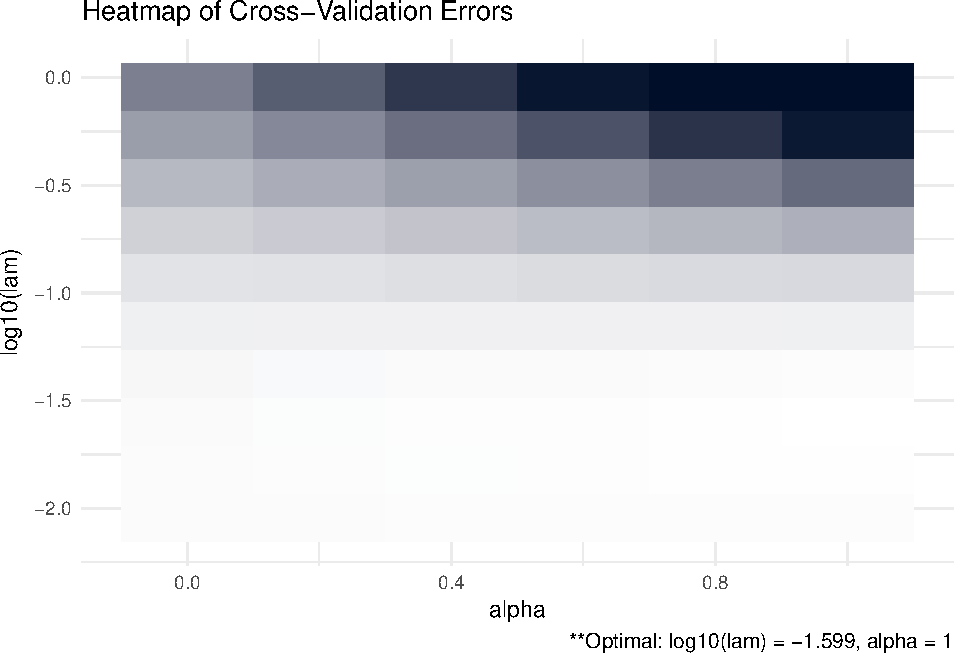
\includegraphics{Manuscript_files/figure-latex/unnamed-chunk-8-1.pdf}
\newpage

\begin{Shaded}
\begin{Highlighting}[]
\CommentTok{# produce line graph for CV errors for ADMMsigma}
\KeywordTok{plot}\NormalTok{(ADMM, }\DataTypeTok{type =} \StringTok{"line"}\NormalTok{)}
\end{Highlighting}
\end{Shaded}

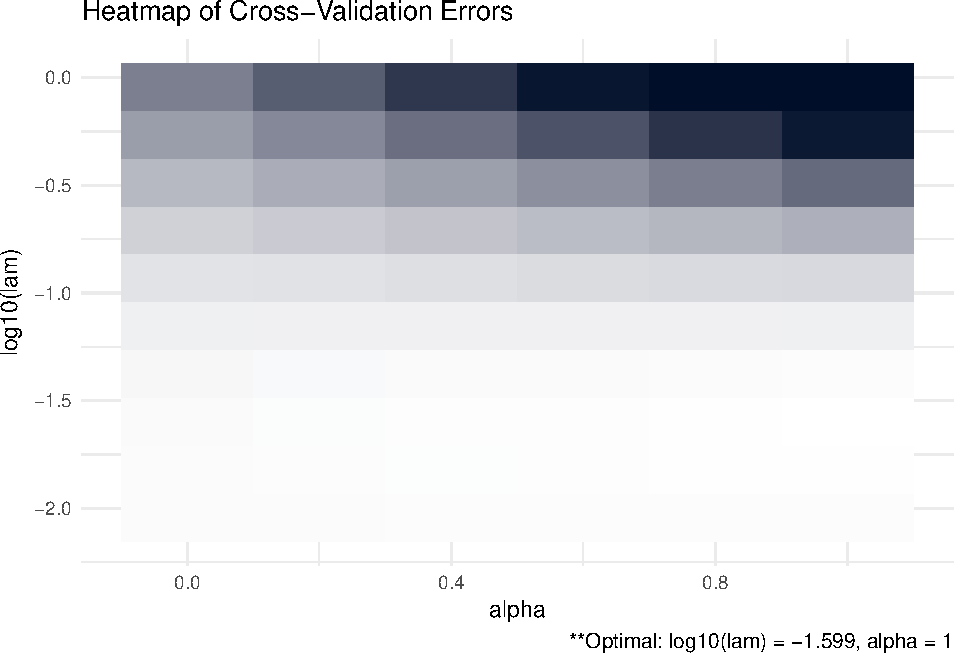
\includegraphics{Manuscript_files/figure-latex/unnamed-chunk-9-1.pdf}
\newpage

\begin{Shaded}
\begin{Highlighting}[]
\CommentTok{# produce CV heat map for RIDGEsigma}
\NormalTok{RIDGE =}\StringTok{ }\KeywordTok{RIDGEsigma}\NormalTok{(X, }\DataTypeTok{lam =} \DecValTok{10}\OperatorTok{^}\KeywordTok{seq}\NormalTok{(}\OperatorTok{-}\DecValTok{8}\NormalTok{, }\DecValTok{8}\NormalTok{, }\FloatTok{0.01}\NormalTok{))}
\KeywordTok{plot}\NormalTok{(RIDGE, }\DataTypeTok{type =} \StringTok{"heatmap"}\NormalTok{)}
\end{Highlighting}
\end{Shaded}

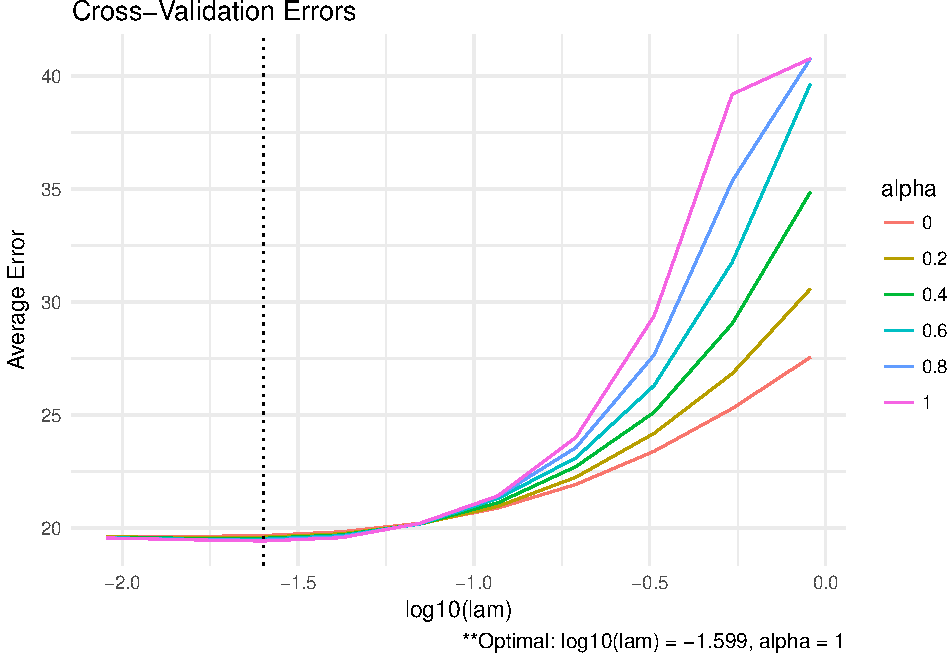
\includegraphics{Manuscript_files/figure-latex/unnamed-chunk-10-1.pdf}

\newpage

\begin{Shaded}
\begin{Highlighting}[]
\CommentTok{# produce line graph for CV errors for RIDGEsigma}
\KeywordTok{plot}\NormalTok{(RIDGE, }\DataTypeTok{type =} \StringTok{"line"}\NormalTok{)}
\end{Highlighting}
\end{Shaded}

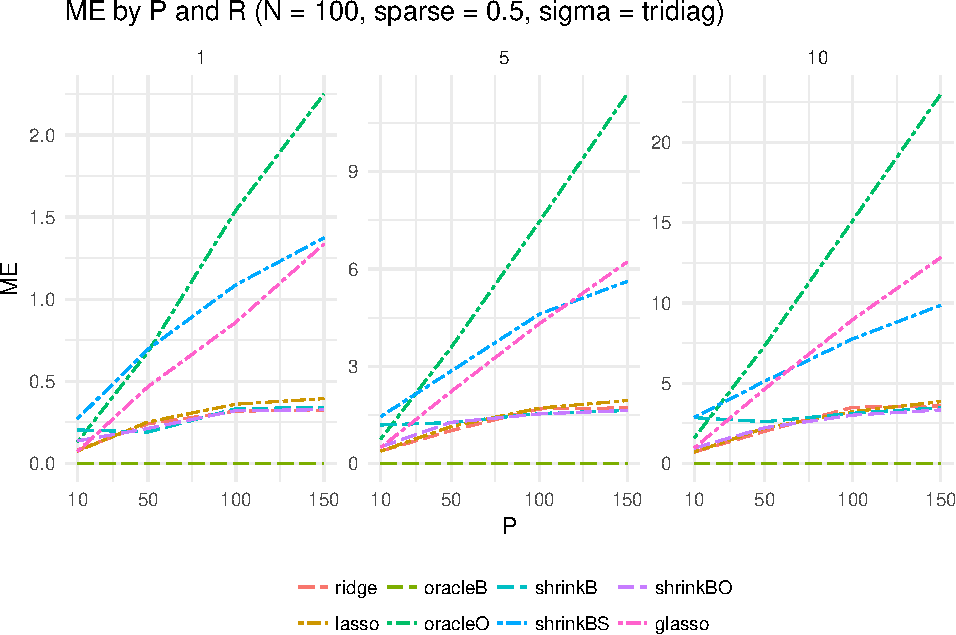
\includegraphics{Manuscript_files/figure-latex/unnamed-chunk-11-1.pdf}

\hypertarget{details}{%
\chapter{Details}\label{details}}

Suppose we want to solve the following optimization problem:

\begin{align*}
  \mbox{minimize } f(x) + g(z) \\
  \mbox{subject to } Ax + Bz = c
\end{align*}

where
\(x \in \mathbb{R}^{n}, z \in \mathbb{R}^{m}, A \in \mathbb{R}^{p \times n}, B \in \mathbb{R}^{p \times m}\),
and \(c \in \mathbb{R}^{p}\). Following \citet{boyd2011distributed}, the
optimization problem will be introduced in vector form though we will
later consider cases where \(x\) and \(z\) are matrices. We will also
assume \(f\) and \(g\) are convex functions. Optimization problems like
this arise naturally in several statistics and machine learning
applications -- particularly regularization methods. For instance, we
could take \(f\) to be the squared error loss, \(g\) to be the
\(l_{2}\)-norm, \(c\) to be equal to zero and \(A\) and \(B\) to be
identity matrices to solve the ridge regression optimization problem.

The \emph{augmented lagrangian} is constructed as follows:

\[ L_{\rho}(x, z, y) = f(x) + g(z) + y^{T}(Ax + Bz - c) + \frac{\rho}{2}\left\| Ax + Bz - c \right\|_{2}^{2} \]

where \(y \in \mathbb{R}^{p}\) is the lagrange multiplier and
\(\rho > 0\) is a scalar. Clearly any minimizer, \(p^{*}\), under the
augmented lagrangian is equivalent to that of the lagrangian since any
feasible point \((x, z)\) satisfies the constraint
\(\rho\left\| Ax + Bz - c \right\|_{2}^{2}/2 = 0\).

\[ p^{*} = inf\left\{ f(x) + g(z) | Ax + Bz = c \right\} \]

The alternating direction method of multipliers (ADMM) algorithm
consists of the following repeated iterations:

\begin{align}
  x^{k + 1} &:= \arg\min_{x}L_{\rho}(x, z^{k}, y^{k}) \\
  z^{k + 1} &:= \arg\min_{z}L_{\rho}(x^{k + 1}, z, y^{k}) \\
  y^{k + 1} &:= y^{k} + \rho(Ax^{k + 1} + Bz^{k + 1} - c)
\end{align}

A more complete introduction to the algorithm -- specifically how it
arose out of \emph{dual ascent} and \emph{method of multipliers} -- can
be found in \citet{boyd2011distributed}.

\vspace{1cm}

\hypertarget{admm-algorithm}{%
\section{ADMM Algorithm}\label{admm-algorithm}}

Now consider the case where \(X_{1}, ..., X_{n}\) are iid
\(N_{p}(\mu, \Sigma)\) random variables and we are tasked with
estimating the precision matrix, denoted \(\Omega \equiv \Sigma^{-1}\).
The maximum likelihood estimator for \(\Omega\) is

\[ \hat{\Omega}_{MLE} = \arg\min_{\Omega \in S_{+}^{p}}\left\{ Tr\left(S\Omega\right) - \log \det\left(\Omega \right) \right\} \]

where \(S = \sum_{i = 1}^{n}(X_{i} - \bar{X})(X_{i} - \bar{X})^{T}/n\)
and \(\bar{X}\) is the sample mean. By setting the gradient equal to
zero, we can show that when the solution exists,
\(\hat{\Omega}_{MLE} = S^{-1}\).

As in regression settings, we can construct a \emph{penalized}
likelihood estimator by adding a penalty term,
\(P\left( \Omega \right)\), to the likelihood:

\[ \hat{\Omega} = \arg\min_{\Omega \in S_{+}^{p}}\left\{ Tr\left(S\Omega\right) - \log \det\left(\Omega \right) + P\left( \Omega \right) \right\} \]

\(P\left( \Omega \right)\) is often of the form
\(P\left(\Omega \right) = \lambda\|\Omega \|_{F}^{2}\) or
\(P\left(\Omega \right) = \|\Omega\|_{1}\) where \(\lambda > 0\),
\(\left\|\cdot \right\|_{F}^{2}\) is the Frobenius norm and we define
\(\left\|A \right\|_{1} = \sum_{i, j} \left| A_{ij} \right|\). These
penalties are the ridge and lasso, respectively. We will, instead, take
\(P\left( \Omega \right) = \lambda\left[\frac{1 - \alpha}{2}\left\| \Omega \right|_{F}^{2} + \alpha\left\| \Omega \right\|_{1} \right]\)
so that the full penalized likelihood is

\[ \hat{\Omega} = \arg\min_{\Omega \in S_{+}^{p}}\left\{ Tr\left(S\Omega\right) - \log \det\left(\Omega \right) + \lambda\left[\frac{1 - \alpha}{2}\left\| \Omega \right|_{F}^{2} + \alpha\left\| \Omega \right\|_{1} \right] \right\} \]

where \(0 \leq \alpha \leq 1\). This \emph{elastic-net} penalty was
explored by Hui Zou and Trevor Hastie \citep{zou2005regularization} and
is identical to the penalty used in the popular penalized regression
package \texttt{glmnet}. Clearly, when \(\alpha = 0\) the elastic-net
reduces to a ridge-type penalty and when \(\alpha = 1\) it reduces to a
lasso-type penalty.

By letting \(f\) be equal to the non-penalized likelihood and \(g\)
equal to \(P\left( \Omega \right)\), our goal is to minimize the full
augmented lagrangian where the constraint is that \(\Omega - Z\) is
equal to zero:

\[ L_{\rho}(\Omega, Z, \Lambda) = f\left(\Omega\right) + g\left(Z\right) + Tr\left[\Lambda\left(\Omega - Z\right)\right] + \frac{\rho}{2}\left\|\Omega - Z\right\|_{F}^{2} \]

The ADMM algorithm for estimating the penalized precision matrix in this
problem is

\begin{align}
  \Omega^{k + 1} &= \arg\min_{\Omega}\left\{ Tr\left(S\Omega\right) - \log\det\left(\Omega\right) + Tr\left[\Lambda^{k}\left(\Omega - Z^{k}\right)\right] + \frac{\rho}{2}\left\| \Omega - Z^{k} \right\|_{F}^{2} \right\} \\
  Z^{k + 1} &= \arg\min_{Z}\left\{ \lambda\left[ \frac{1 - \alpha}{2}\left\| Z \right\|_{F}^{2} + \alpha\left\| Z \right\|_{1} \right] + Tr\left[\Lambda^{k}\left(\Omega^{k + 1} - Z\right)\right] + \frac{\rho}{2}\left\| \Omega^{k + 1} - Z \right\|_{F}^{2} \right\} \\
  \Lambda^{k + 1} &= \Lambda^{k} + \rho\left( \Omega^{k + 1} - Z^{k + 1} \right)
\end{align}

\vspace{1cm}

\hypertarget{scaled-form-admm}{%
\section{Scaled-Form ADMM}\label{scaled-form-admm}}

An alternate form of the ADMM algorithm can constructed by scaling the
dual variable (\(\Lambda^{k}\)). Let us define
\(R^{k} = \Omega - Z^{k}\) and \(U^{k} = \Lambda^{k}/\rho\).

\begin{align*}
  Tr\left[ \Lambda^{k}\left( \Omega - Z^{k} \right) \right] + \frac{\rho}{2}\left\| \Omega - Z^{k} \right\|_{F}^{2} &= Tr\left[ \Lambda^{k}R^{k} \right] + \frac{\rho}{2}\left\| R^{k} \right\|_{F}^{2} \\
  &= \frac{\rho}{2}\left\| R^{k} + \Lambda^{k}/\rho \right\|_{F}^{2} - \frac{\rho}{2}\left\| \Lambda^{k}/\rho \right\|_{F}^{2} \\
  &= \frac{\rho}{2}\left\| R^{k} + U^{k} \right\|_{F}^{2} - \frac{\rho}{2}\left\| U^{k} \right\|_{F}^{2}
\end{align*}

Therefore, the condensed-form ADMM algorithm can now be written as

\begin{align}
  \Omega^{k + 1} &= \arg\min_{\Omega}\left\{ Tr\left(S\Omega\right) - \log\det\left(\Omega\right) + \frac{\rho}{2}\left\| \Omega - Z^{k} + U^{k} \right\|_{F}^{2} \right\} \\
  Z^{k + 1} &= \arg\min_{Z}\left\{ \lambda\left[ \frac{1 - \alpha}{2}\left\| Z \right\|_{F}^{2} + \alpha\left\| Z \right\|_{1} \right] + \frac{\rho}{2}\left\| \Omega^{k + 1} - Z + U^{k} \right\|_{F}^{2} \right\} \\
  U^{k + 1} &= U^{k} + \Omega^{k + 1} - Z^{k + 1}
\end{align}

And more generally (in vector form),

\begin{align}
  x^{k + 1} &= \arg\min_{x}\left\{ f(x) + \frac{\rho}{2}\left\| Ax + Bz^{k} - c + u^{k} \right\|_{2}^{2} \right\} \\
  z^{k + 1} &= \arg\min_{z}\left\{ g(z) + \frac{\rho}{2}\left\| Ax^{k + 1} + Bz - c + u^{k} \right\|_{2}^{2} \right\} \\
  u^{k + 1} &= u^{k} + Ax^{k + 1} + Bz^{k + 1} - c
\end{align}

Note that there are limitations to using this method. Because the dual
variable is scaled by \(\rho\) (the step size), this form limits one to
using a constant step size without making further adjustments to
\(U^{k}\). It has been shown in the literature that a dynamic step size
can significantly reduce the number of iterations required for
convergence.

\vspace{1cm}

\hypertarget{algorithm}{%
\section{Algorithm}\label{algorithm}}

\begin{align*}
  \Omega^{k + 1} &= \arg\min_{\Omega}\left\{ Tr\left(S\Omega\right) - \log\det\left(\Omega\right) + Tr\left[\Lambda^{k}\left(\Omega - Z^{k}\right)\right] + \frac{\rho}{2}\left\| \Omega - Z^{k} \right\|_{F}^{2} \right\} \\
  Z^{k + 1} &= \arg\min_{Z}\left\{ \lambda\left[ \frac{1 - \alpha}{2}\left\| Z \right\|_{F}^{2} + \alpha\left\| Z \right\|_{1} \right] + Tr\left[\Lambda^{k}\left(\Omega^{k + 1} - Z\right)\right] + \frac{\rho}{2}\left\| \Omega^{k + 1} - Z \right\|_{F}^{2} \right\} \\
  \Lambda^{k + 1} &= \Lambda^{k} + \rho\left( \Omega^{k + 1} - Z^{k + 1} \right)
\end{align*}

\vspace{1cm}

Initialize \(Z^{0}, \Lambda^{0}\), and \(\rho\). Iterate the following
three steps until convergence:

\begin{enumerate}
\def\labelenumi{\arabic{enumi}.}
\tightlist
\item
  Decompose \(S + \Lambda^{k} - \rho Z^{k} = VQV^{T}\) via spectral
  decomposition.
\end{enumerate}

\[ \Omega^{k + 1} = \frac{1}{2\rho}V\left[ -Q + \left( Q^{2} + 4\rho I_{p} \right)^{1/2} \right]V^{T} \]

\begin{enumerate}
\def\labelenumi{\arabic{enumi}.}
\setcounter{enumi}{1}
\tightlist
\item
  Elementwise soft-thresholding for all \(i = 1,..., p\) and
  \(j = 1,..., p\).
\end{enumerate}

\begin{align*}
Z_{ij}^{k + 1} &= \frac{1}{\lambda(1 - \alpha) + \rho}Sign\left(\rho\Omega_{ij}^{k + 1} + \Lambda_{ij}^{k}\right)\left( \left| \rho\Omega_{ij}^{k + 1} + \Lambda_{ij}^{k} \right| - \lambda\alpha \right)_{+} \\
&= \frac{1}{\lambda(1 - \alpha) + \rho}Soft\left(\rho\Omega_{ij}^{k + 1} + \Lambda_{ij}^{k}, \lambda\alpha\right)
\end{align*}

\begin{enumerate}
\def\labelenumi{\arabic{enumi}.}
\setcounter{enumi}{2}
\tightlist
\item
  Update \(\Lambda^{k + 1}\).
\end{enumerate}

\[ \Lambda^{k + 1} = \Lambda^{k} + \rho\left( \Omega^{k + 1} - Z^{k + 1} \right) \]

\vspace{1cm}

\hypertarget{proof-of-1}{%
\subsection{Proof of (1):}\label{proof-of-1}}

\[ \Omega^{k + 1} = \arg\min_{\Omega}\left\{ Tr\left(S\Omega\right) - \log\det\left(\Omega\right) + Tr\left[\Lambda^{k}\left(\Omega - Z^{k}\right)\right] + \frac{\rho}{2}\left\| \Omega - Z^{k} \right\|_{F}^{2} \right\} \]

\begin{align*}
  \nabla_{\Omega}&\left\{ Tr\left(S\Omega\right) - \log\det\left(\Omega\right) + Tr\left[\Lambda^{k}\left(\Omega - Z^{k}\right)\right] + \frac{\rho}{2}\left\| \Omega - Z^{k} \right\|_{F}^{2} \right\} \\
  &= S - \Omega^{-1} + \Lambda^{k} + \rho\left( \Omega - Z^{k} \right)
\end{align*}

Set the gradient equal to zero and decompose \(\Omega = VDV^{T}\) where
\(D\) is a diagonal matrix with diagonal elements equal to the eigen
values of \(\Omega\) and \(V\) is the matrix with corresponding eigen
vectors as columns.

\[ S + \Lambda^{k} - \rho Z^{k} = \Omega^{-1} - \rho \Omega = VD^{-1}V^{T} - \rho VDV^{T} =  V\left(D^{-1} - \rho D\right)V^{T} \]

This equivalence implies that

\[ \phi_{j}\left( S + \Lambda^{k} - \rho Z^{k} \right) = \frac{1}{\phi_{j}(\Omega^{k + 1})} - \rho\phi_{j}(\Omega^{k + 1}) \]

where \(\phi_{j}(\cdot)\) is the \(j\)th eigen value.

\begin{align*}
  &\Rightarrow \rho\phi_{j}^{2}(\Omega^{k + 1}) + \phi_{j}\left( S + \Lambda^{k} - \rho Z^{k} \right)\phi_{j}(\Omega^{k + 1}) - 1 = 0 \\
  &\Rightarrow \phi_{j}(\Omega^{k + 1}) = \frac{-\phi_{j}(S + \Lambda^{k} - \rho Z^{k}) \pm \sqrt{\phi_{j}^{2}(S + \Lambda^{k} - \rho Z^{k}) + 4\rho}}{2\rho}
\end{align*}

In summary, if we decompose \(S + \Lambda^{k} - \rho Z^{k} = VQV^{T}\)
then

\[ \Omega^{k + 1} = \frac{1}{2\rho}V\left[ -Q + (Q^{2} + 4\rho I_{p})^{1/2}\right] V^{T} \]

\vspace{1cm}

\hypertarget{proof-of-2}{%
\subsection{Proof of (2)}\label{proof-of-2}}

\[ Z^{k + 1} = \arg\min_{Z}\left\{ \lambda\left[ \frac{1 - \alpha}{2}\left\| Z \right\|_{F}^{2} + \alpha\left\| Z \right\|_{1} \right] + Tr\left[\Lambda^{k}\left(\Omega^{k + 1} - Z\right)\right] + \frac{\rho}{2}\left\| \Omega^{k + 1} - Z \right\|_{F}^{2} \right\} \]

\begin{align*}
  \partial&\left\{ \lambda\left[ \frac{1 - \alpha}{2}\left\| Z \right\|_{F}^{2} + \alpha\left\| Z \right\|_{1} \right] + Tr\left[\Lambda^{k}\left(\Omega^{k + 1} - Z\right)\right] + \frac{\rho}{2}\left\| \Omega^{k + 1} - Z \right\|_{F}^{2} \right\} \\
  &= \partial\left\{ \lambda\left[ \frac{1 - \alpha}{2}\left\| Z \right\|_{F}^{2} + \alpha\left\| Z \right\|_{1} \right] + Tr\left[\Lambda^{k}\left(\Omega^{k + 1} - Z\right)\right]\right\} + \nabla_{\Omega}\left\{\frac{\rho}{2}\left\| \Omega^{k + 1} - Z \right\|_{F}^{2} \right\} \\
  &= \lambda(1 - \alpha)Z + Sign(Z)\lambda\alpha - \Lambda^{k} - \rho\left( \Omega^{k + 1} - Z \right)
\end{align*}

where \(Sign(Z)\) is the elementwise Sign operator. By setting the
gradient/sub-differential equal to zero, we arrive at the following
equivalence:

\[ Z_{ij} = \frac{1}{\lambda(1 - \alpha) + \rho}\left( \rho \Omega_{ij}^{k + 1} + \Lambda_{ij}^{k} - Sign(Z_{ij})\lambda\alpha \right) \]

for all \(i = 1,..., p\) and \(j = 1,..., p\). We observe two scenarios:

\begin{itemize}
\tightlist
\item
  If \(Z_{ij} > 0\) then
\end{itemize}

\[ \rho\Omega_{ij}^{k + 1} + \Lambda_{ij}^{k} > \lambda\alpha \]

\begin{itemize}
\tightlist
\item
  If \(Z_{ij} < 0\) then
\end{itemize}

\[ \rho\Omega_{ij}^{k + 1} + \Lambda_{ij}^{k} < -\lambda\alpha \]

This implies that
\(Sign(Z_{ij}) = Sign(\rho\Omega_{ij}^{k + 1} + \Lambda_{ij}^{k})\).
Putting all the pieces together, we arrive at

\begin{align*}
Z_{ij}^{k + 1} &= \frac{1}{\lambda(1 - \alpha) + \rho}Sign\left(\rho\Omega_{ij}^{k + 1} + \Lambda_{ij}^{k}\right)\left( \left| \rho\Omega_{ij}^{k + 1} + \Lambda_{ij}^{k} \right| - \lambda\alpha \right)_{+} \\
&= \frac{1}{\lambda(1 - \alpha) + \rho}Soft\left(\rho\Omega_{ij}^{k + 1} + \Lambda_{ij}^{k}, \lambda\alpha\right)
\end{align*}

where \(Soft\) is the soft-thresholding function.

\newpage

\hypertarget{references}{%
\section{References}\label{references}}

\hypertarget{simulations}{%
\chapter{Simulations}\label{simulations}}

In the simulations below we generated data from a number of oracle
precision matrices with various structures. For each data-generating
procedure, the \texttt{ADMMsigma()} function was run using 5-fold cross
validation. After 20 replications, the cross validation errors were
totalled and the optimal tuning parameters were selected (results in the
top figure). These results are compared with the Kullback Leibler (KL)
losses between the estimates and the oracle precision matrix (bottom
figure). We can see below that our cross validation procedure choosing
tuning parameters close to the optimal parameters.

\newpage

\hypertarget{compound-symmetric-p-100-n-50}{%
\subsection{Compound Symmetric: P = 100, N =
50}\label{compound-symmetric-p-100-n-50}}

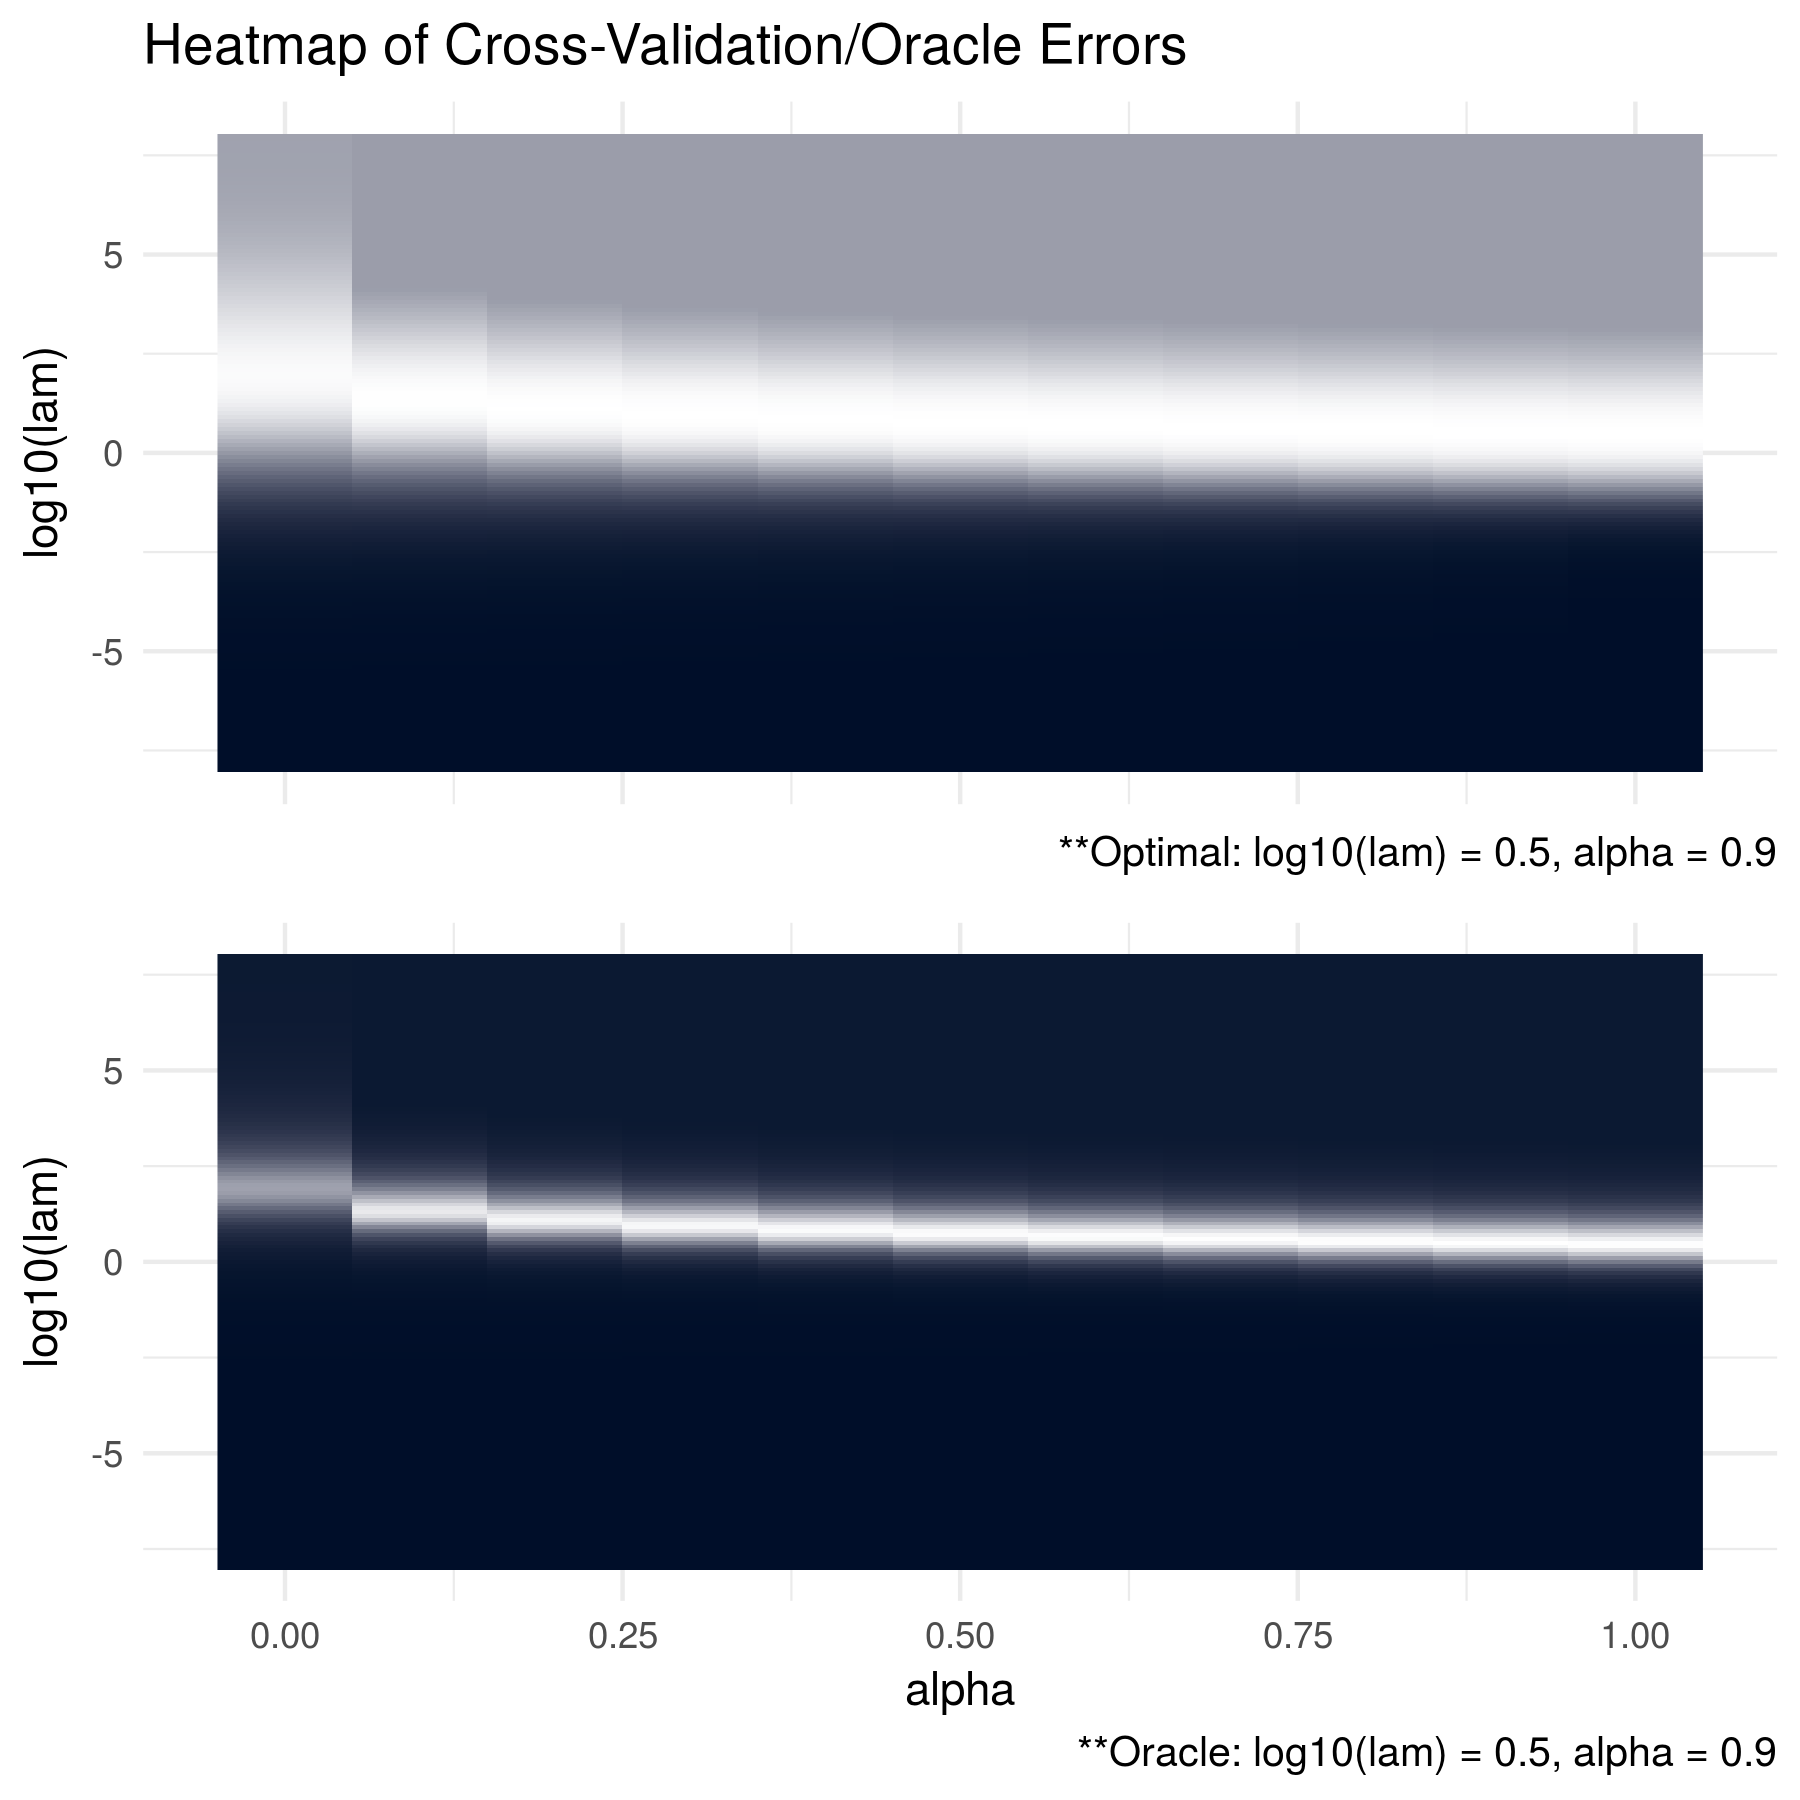
\includegraphics{images/compound_N50_P100.png}

\vspace{0.5cm}

\begin{Shaded}
\begin{Highlighting}[]
\CommentTok{# oracle precision matrix}
\NormalTok{Omega =}\StringTok{ }\KeywordTok{matrix}\NormalTok{(}\FloatTok{0.9}\NormalTok{, }\DataTypeTok{ncol =} \DecValTok{100}\NormalTok{, }\DataTypeTok{nrow =} \DecValTok{100}\NormalTok{)}
\KeywordTok{diag}\NormalTok{(}\DataTypeTok{Omega =} \DecValTok{1}\NormalTok{)}

\CommentTok{# generate covariance matrix}
\NormalTok{S =}\StringTok{ }\KeywordTok{qr.solve}\NormalTok{(Omega)}

\CommentTok{# generate data}
\NormalTok{Z =}\StringTok{ }\KeywordTok{matrix}\NormalTok{(}\KeywordTok{rnorm}\NormalTok{(}\DecValTok{100} \OperatorTok{*}\StringTok{ }\DecValTok{50}\NormalTok{), }\DataTypeTok{nrow =} \DecValTok{50}\NormalTok{, }\DataTypeTok{ncol =} \DecValTok{100}\NormalTok{)}
\NormalTok{out =}\StringTok{ }\KeywordTok{eigen}\NormalTok{(S, }\DataTypeTok{symmetric =} \OtherTok{TRUE}\NormalTok{)}
\NormalTok{S.sqrt =}\StringTok{ }\NormalTok{out}\OperatorTok{$}\NormalTok{vectors }\OperatorTok\StringTok{ }\KeywordTok{diag}\NormalTok{(out}\OperatorTok{$}\NormalTok{values}\OperatorTok{^}\FloatTok{0.5}\NormalTok{) }\OperatorTok\StringTok{ }\KeywordTok{t}\NormalTok{(out}\OperatorTok{$}\NormalTok{vectors)}
\NormalTok{X =}\StringTok{ }\NormalTok{Z }\OperatorTok\StringTok{ }\NormalTok{S.sqrt}
\end{Highlighting}
\end{Shaded}

\newpage

\hypertarget{compound-symmetric-p-10-n-1000}{%
\subsection{Compound Symmetric: P = 10, N =
1000}\label{compound-symmetric-p-10-n-1000}}

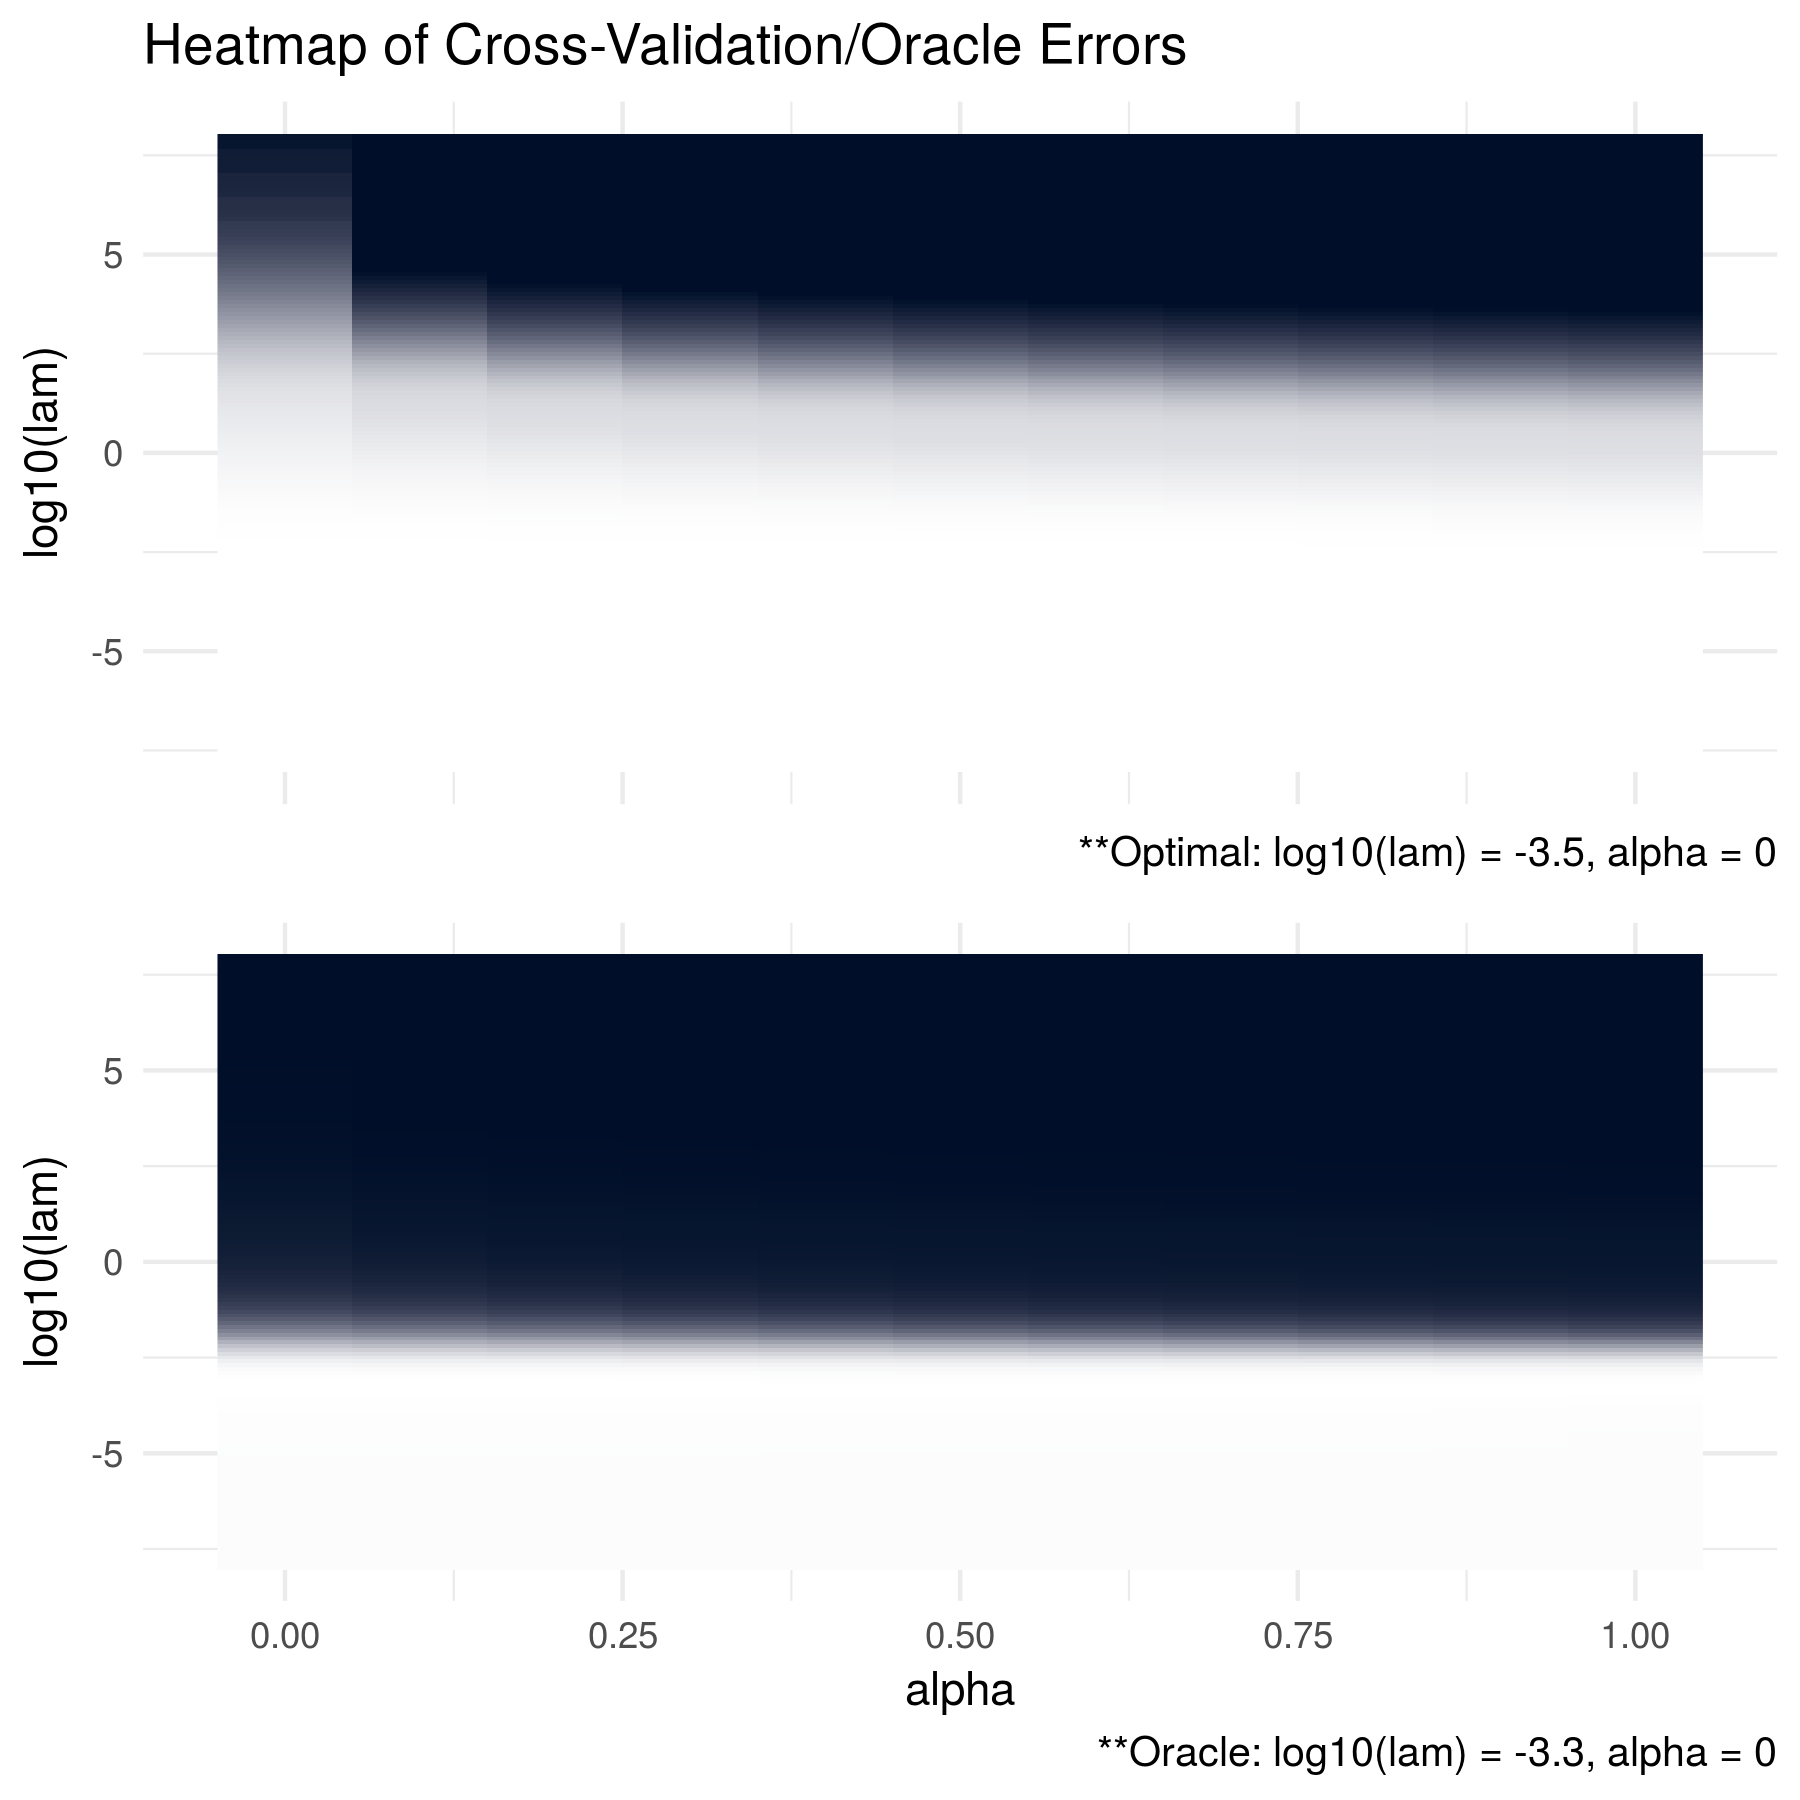
\includegraphics{images/compound_N1000_P10.png}

\vspace{0.5cm}

\begin{Shaded}
\begin{Highlighting}[]
\CommentTok{# oracle precision matrix}
\NormalTok{Omega =}\StringTok{ }\KeywordTok{matrix}\NormalTok{(}\FloatTok{0.9}\NormalTok{, }\DataTypeTok{ncol =} \DecValTok{10}\NormalTok{, }\DataTypeTok{nrow =} \DecValTok{10}\NormalTok{)}
\KeywordTok{diag}\NormalTok{(}\DataTypeTok{Omega =} \DecValTok{1}\NormalTok{)}

\CommentTok{# generate covariance matrix}
\NormalTok{S =}\StringTok{ }\KeywordTok{qr.solve}\NormalTok{(Omega)}

\CommentTok{# generate data}
\NormalTok{Z =}\StringTok{ }\KeywordTok{matrix}\NormalTok{(}\KeywordTok{rnorm}\NormalTok{(}\DecValTok{10} \OperatorTok{*}\StringTok{ }\DecValTok{1000}\NormalTok{), }\DataTypeTok{nrow =} \DecValTok{1000}\NormalTok{, }\DataTypeTok{ncol =} \DecValTok{10}\NormalTok{)}
\NormalTok{out =}\StringTok{ }\KeywordTok{eigen}\NormalTok{(S, }\DataTypeTok{symmetric =} \OtherTok{TRUE}\NormalTok{)}
\NormalTok{S.sqrt =}\StringTok{ }\NormalTok{out}\OperatorTok{$}\NormalTok{vectors }\OperatorTok\StringTok{ }\KeywordTok{diag}\NormalTok{(out}\OperatorTok{$}\NormalTok{values}\OperatorTok{^}\FloatTok{0.5}\NormalTok{) }\OperatorTok\StringTok{ }\KeywordTok{t}\NormalTok{(out}\OperatorTok{$}\NormalTok{vectors)}
\NormalTok{X =}\StringTok{ }\NormalTok{Z }\OperatorTok\StringTok{ }\NormalTok{S.sqrt}
\end{Highlighting}
\end{Shaded}

\newpage

\hypertarget{dense-p-100-n-50}{%
\subsection{Dense: P = 100, N = 50}\label{dense-p-100-n-50}}

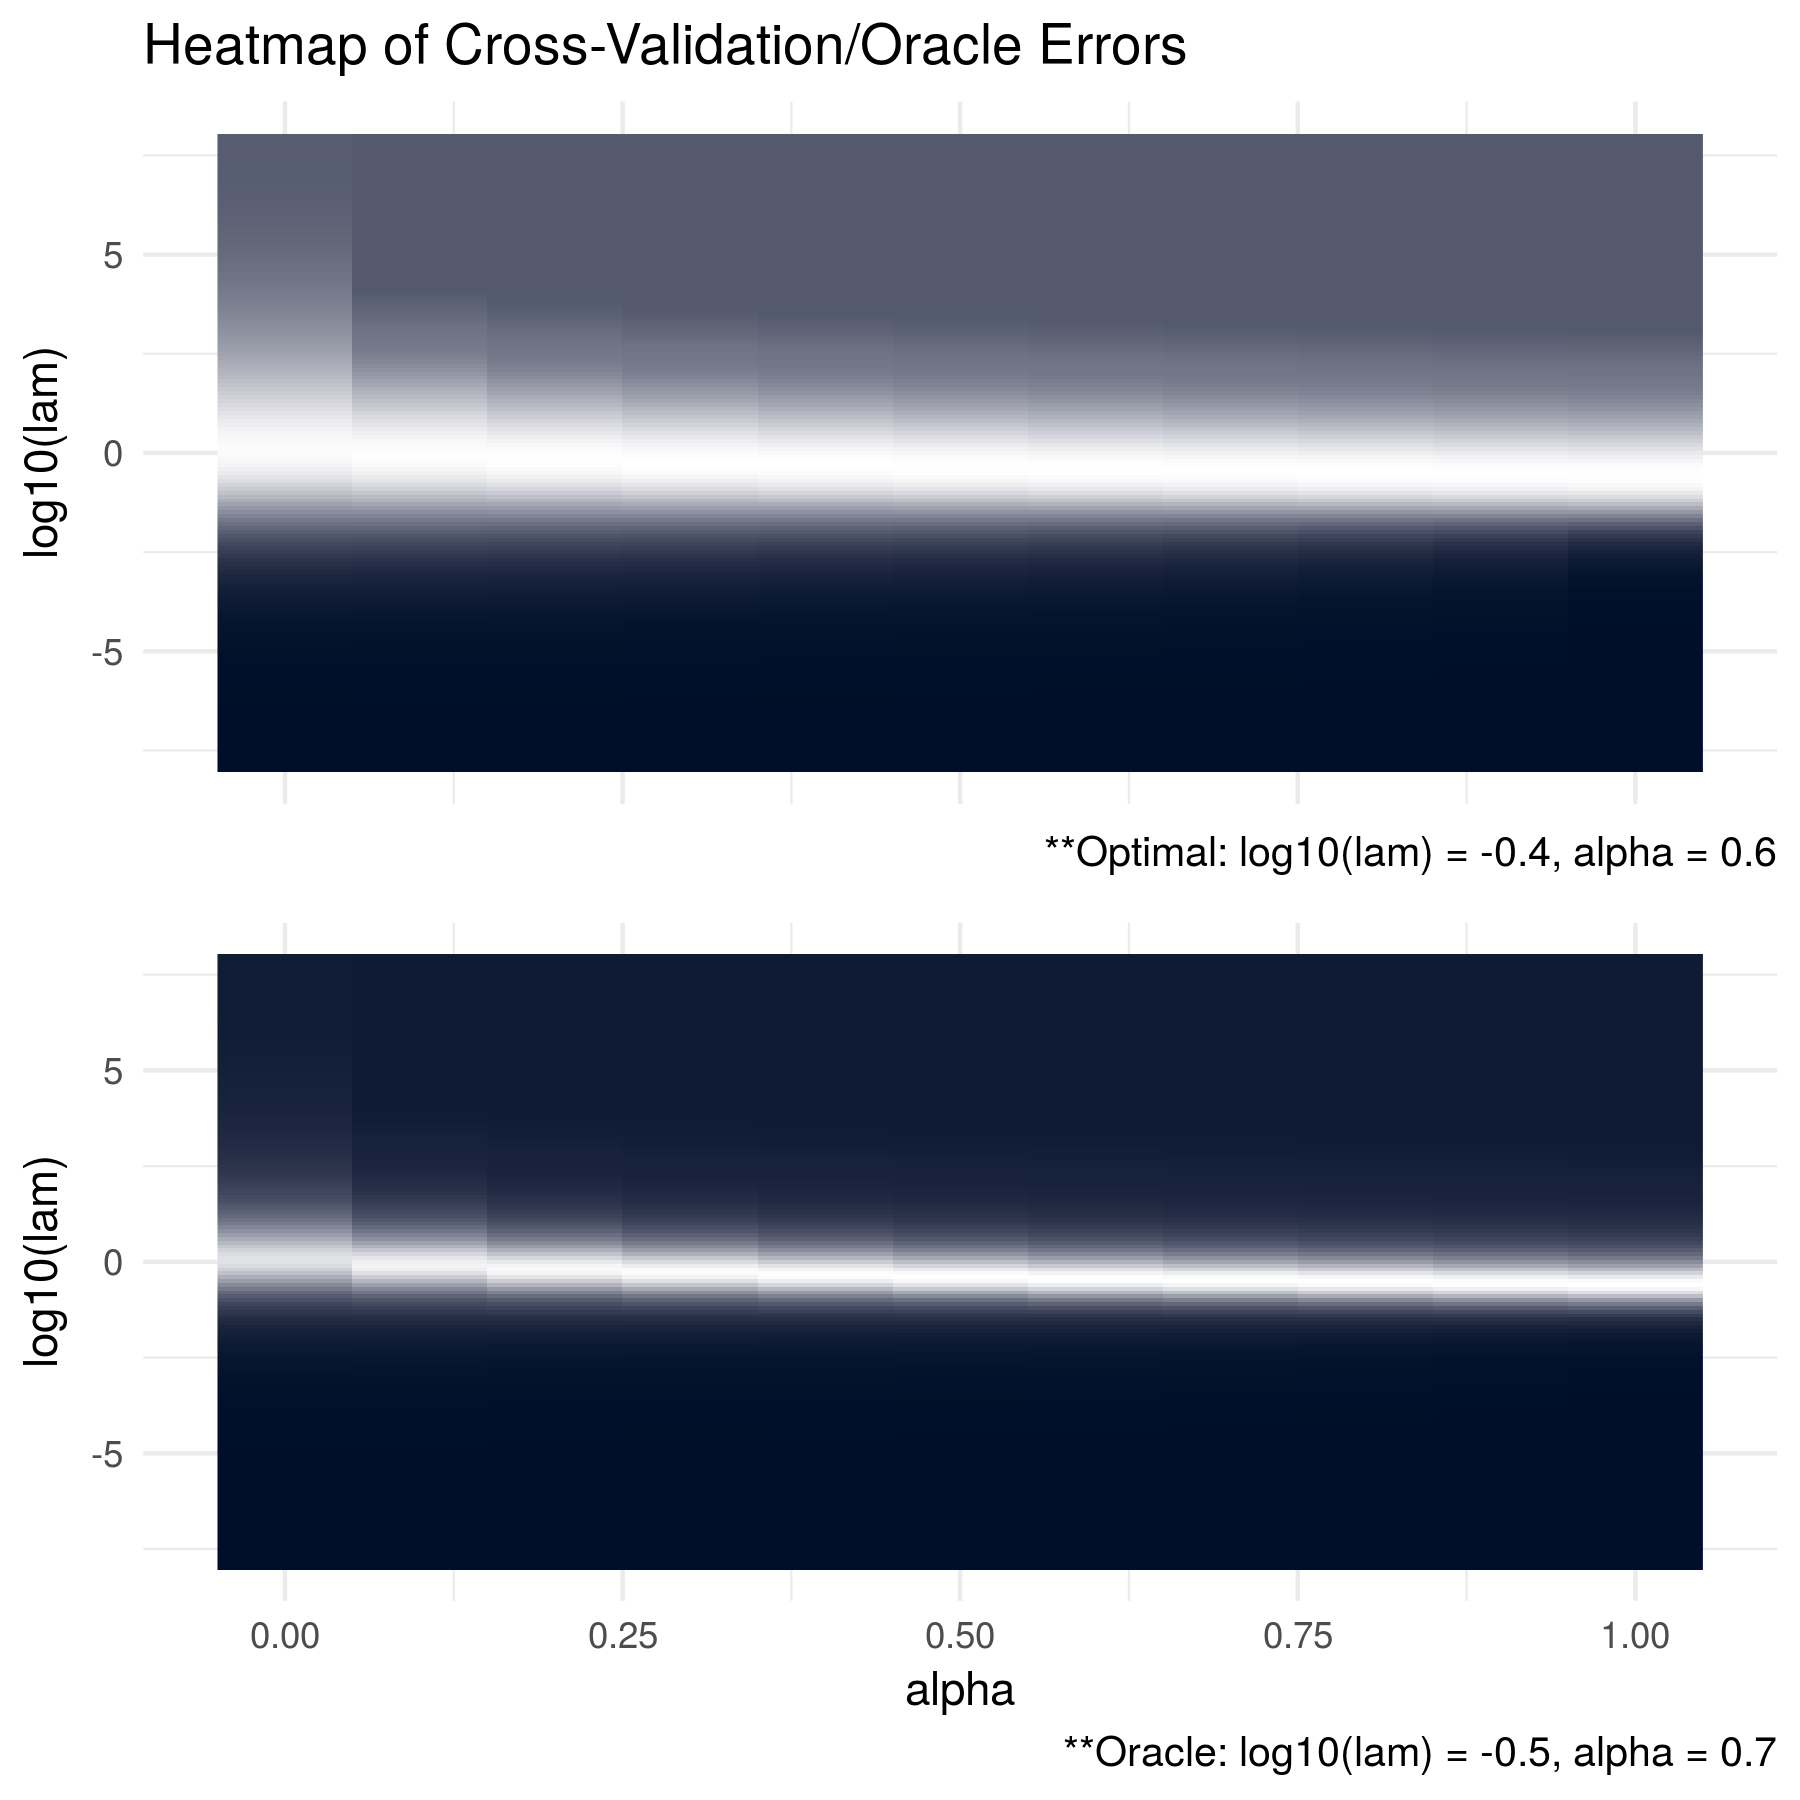
\includegraphics{images/repsKLdenseQR_N50_P100.png}

\vspace{0.5cm}

\begin{Shaded}
\begin{Highlighting}[]
\CommentTok{# generate eigen values}
\NormalTok{eigen =}\StringTok{ }\KeywordTok{c}\NormalTok{(}\KeywordTok{rep}\NormalTok{(}\DecValTok{1000}\NormalTok{, }\DecValTok{5}\NormalTok{, }\KeywordTok{rep}\NormalTok{(}\DecValTok{1}\NormalTok{, }\DecValTok{100} \OperatorTok{-}\StringTok{ }\DecValTok{5}\NormalTok{)))}

\CommentTok{# randomly generate orthogonal basis (via QR)}
\NormalTok{Q =}\StringTok{ }\KeywordTok{matrix}\NormalTok{(}\KeywordTok{rnorm}\NormalTok{(}\DecValTok{100}\OperatorTok{*}\DecValTok{100}\NormalTok{), }\DataTypeTok{nrow =} \DecValTok{100}\NormalTok{, }\DataTypeTok{ncol =} \DecValTok{100}\NormalTok{) }\OperatorTok\StringTok{ }\NormalTok{qr }\OperatorTok\StringTok{ }\NormalTok{qr.Q}

\CommentTok{# generate covariance matrix}
\NormalTok{S =}\StringTok{ }\NormalTok{Q }\OperatorTok\StringTok{ }\KeywordTok{diag}\NormalTok{(eigen) }\OperatorTok\StringTok{ }\KeywordTok{t}\NormalTok{(Q)}

\CommentTok{# generate data}
\NormalTok{Z =}\StringTok{ }\KeywordTok{matrix}\NormalTok{(}\KeywordTok{rnorm}\NormalTok{(}\DecValTok{100}\OperatorTok{*}\DecValTok{50}\NormalTok{), }\DataTypeTok{nrow =} \DecValTok{50}\NormalTok{, }\DataTypeTok{ncol =} \DecValTok{100}\NormalTok{)}
\NormalTok{out =}\StringTok{ }\KeywordTok{eigen}\NormalTok{(S, }\DataTypeTok{symmetric =} \OtherTok{TRUE}\NormalTok{)}
\NormalTok{S.sqrt =}\StringTok{ }\NormalTok{out}\OperatorTok{$}\NormalTok{vectors }\OperatorTok\StringTok{ }\KeywordTok{diag}\NormalTok{(out}\OperatorTok{$}\NormalTok{values}\OperatorTok{^}\FloatTok{0.5}\NormalTok{) }\OperatorTok\StringTok{ }\KeywordTok{t}\NormalTok{(out}\OperatorTok{$}\NormalTok{vectors)}
\NormalTok{X =}\StringTok{ }\NormalTok{Z }\OperatorTok\StringTok{ }\NormalTok{S.sqrt}
\end{Highlighting}
\end{Shaded}

\newpage

\hypertarget{dense-p-10-n-50}{%
\subsection{Dense: P = 10, N = 50}\label{dense-p-10-n-50}}

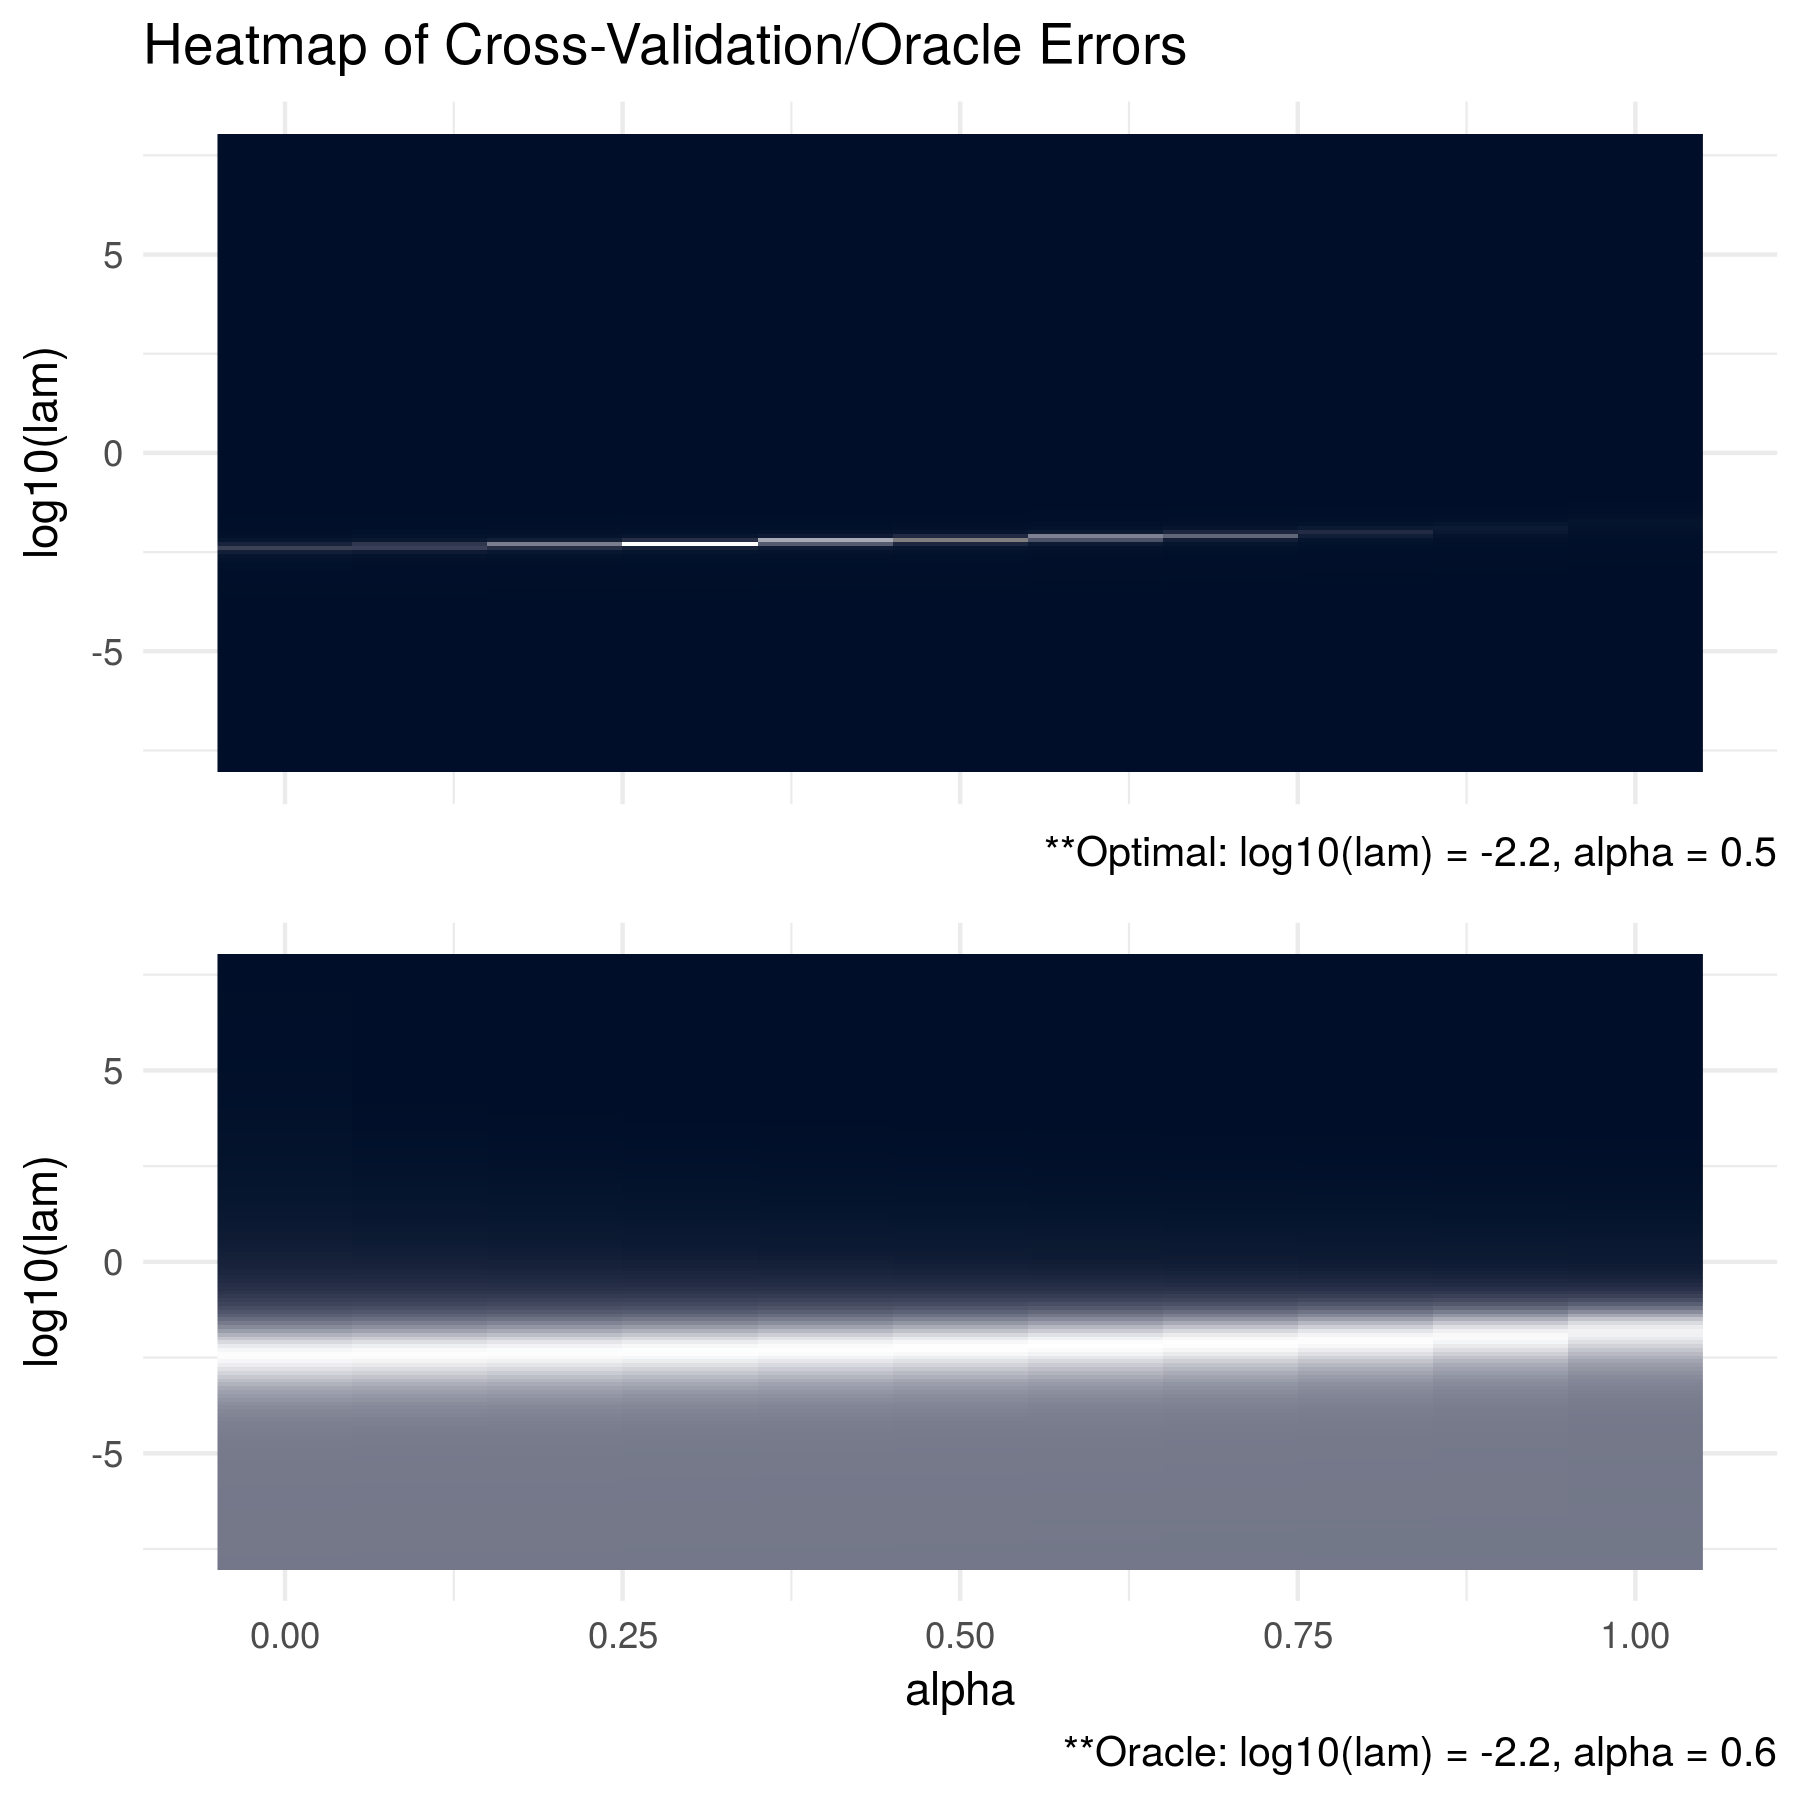
\includegraphics{images/repsKLdense_N50_P10.png}

\vspace{0.5cm}

\begin{Shaded}
\begin{Highlighting}[]
\CommentTok{# generate eigen values}
\NormalTok{eigen =}\StringTok{ }\KeywordTok{c}\NormalTok{(}\KeywordTok{rep}\NormalTok{(}\DecValTok{1000}\NormalTok{, }\DecValTok{5}\NormalTok{, }\KeywordTok{rep}\NormalTok{(}\DecValTok{1}\NormalTok{, }\DecValTok{10} \OperatorTok{-}\StringTok{ }\DecValTok{5}\NormalTok{)))}

\CommentTok{# randomly generate orthogonal basis (via QR)}
\NormalTok{Q =}\StringTok{ }\KeywordTok{matrix}\NormalTok{(}\KeywordTok{rnorm}\NormalTok{(}\DecValTok{10}\OperatorTok{*}\DecValTok{10}\NormalTok{), }\DataTypeTok{nrow =} \DecValTok{10}\NormalTok{, }\DataTypeTok{ncol =} \DecValTok{10}\NormalTok{) }\OperatorTok\StringTok{ }\NormalTok{qr }\OperatorTok\StringTok{ }\NormalTok{qr.Q}

\CommentTok{# generate covariance matrix}
\NormalTok{S =}\StringTok{ }\NormalTok{Q }\OperatorTok\StringTok{ }\KeywordTok{diag}\NormalTok{(eigen) }\OperatorTok\StringTok{ }\KeywordTok{t}\NormalTok{(Q)}

\CommentTok{# generate data}
\NormalTok{Z =}\StringTok{ }\KeywordTok{matrix}\NormalTok{(}\KeywordTok{rnorm}\NormalTok{(}\DecValTok{10}\OperatorTok{*}\DecValTok{50}\NormalTok{), }\DataTypeTok{nrow =} \DecValTok{50}\NormalTok{, }\DataTypeTok{ncol =} \DecValTok{10}\NormalTok{)}
\NormalTok{out =}\StringTok{ }\KeywordTok{eigen}\NormalTok{(S, }\DataTypeTok{symmetric =} \OtherTok{TRUE}\NormalTok{)}
\NormalTok{S.sqrt =}\StringTok{ }\NormalTok{out}\OperatorTok{$}\NormalTok{vectors }\OperatorTok\StringTok{ }\KeywordTok{diag}\NormalTok{(out}\OperatorTok{$}\NormalTok{values}\OperatorTok{^}\FloatTok{0.5}\NormalTok{) }\OperatorTok\StringTok{ }\KeywordTok{t}\NormalTok{(out}\OperatorTok{$}\NormalTok{vectors)}
\NormalTok{X =}\StringTok{ }\NormalTok{Z }\OperatorTok\StringTok{ }\NormalTok{S.sqrt}
\end{Highlighting}
\end{Shaded}

\newpage

\hypertarget{tridiagonal-p-100-n-50}{%
\subsection{Tridiagonal: P = 100, N = 50}\label{tridiagonal-p-100-n-50}}

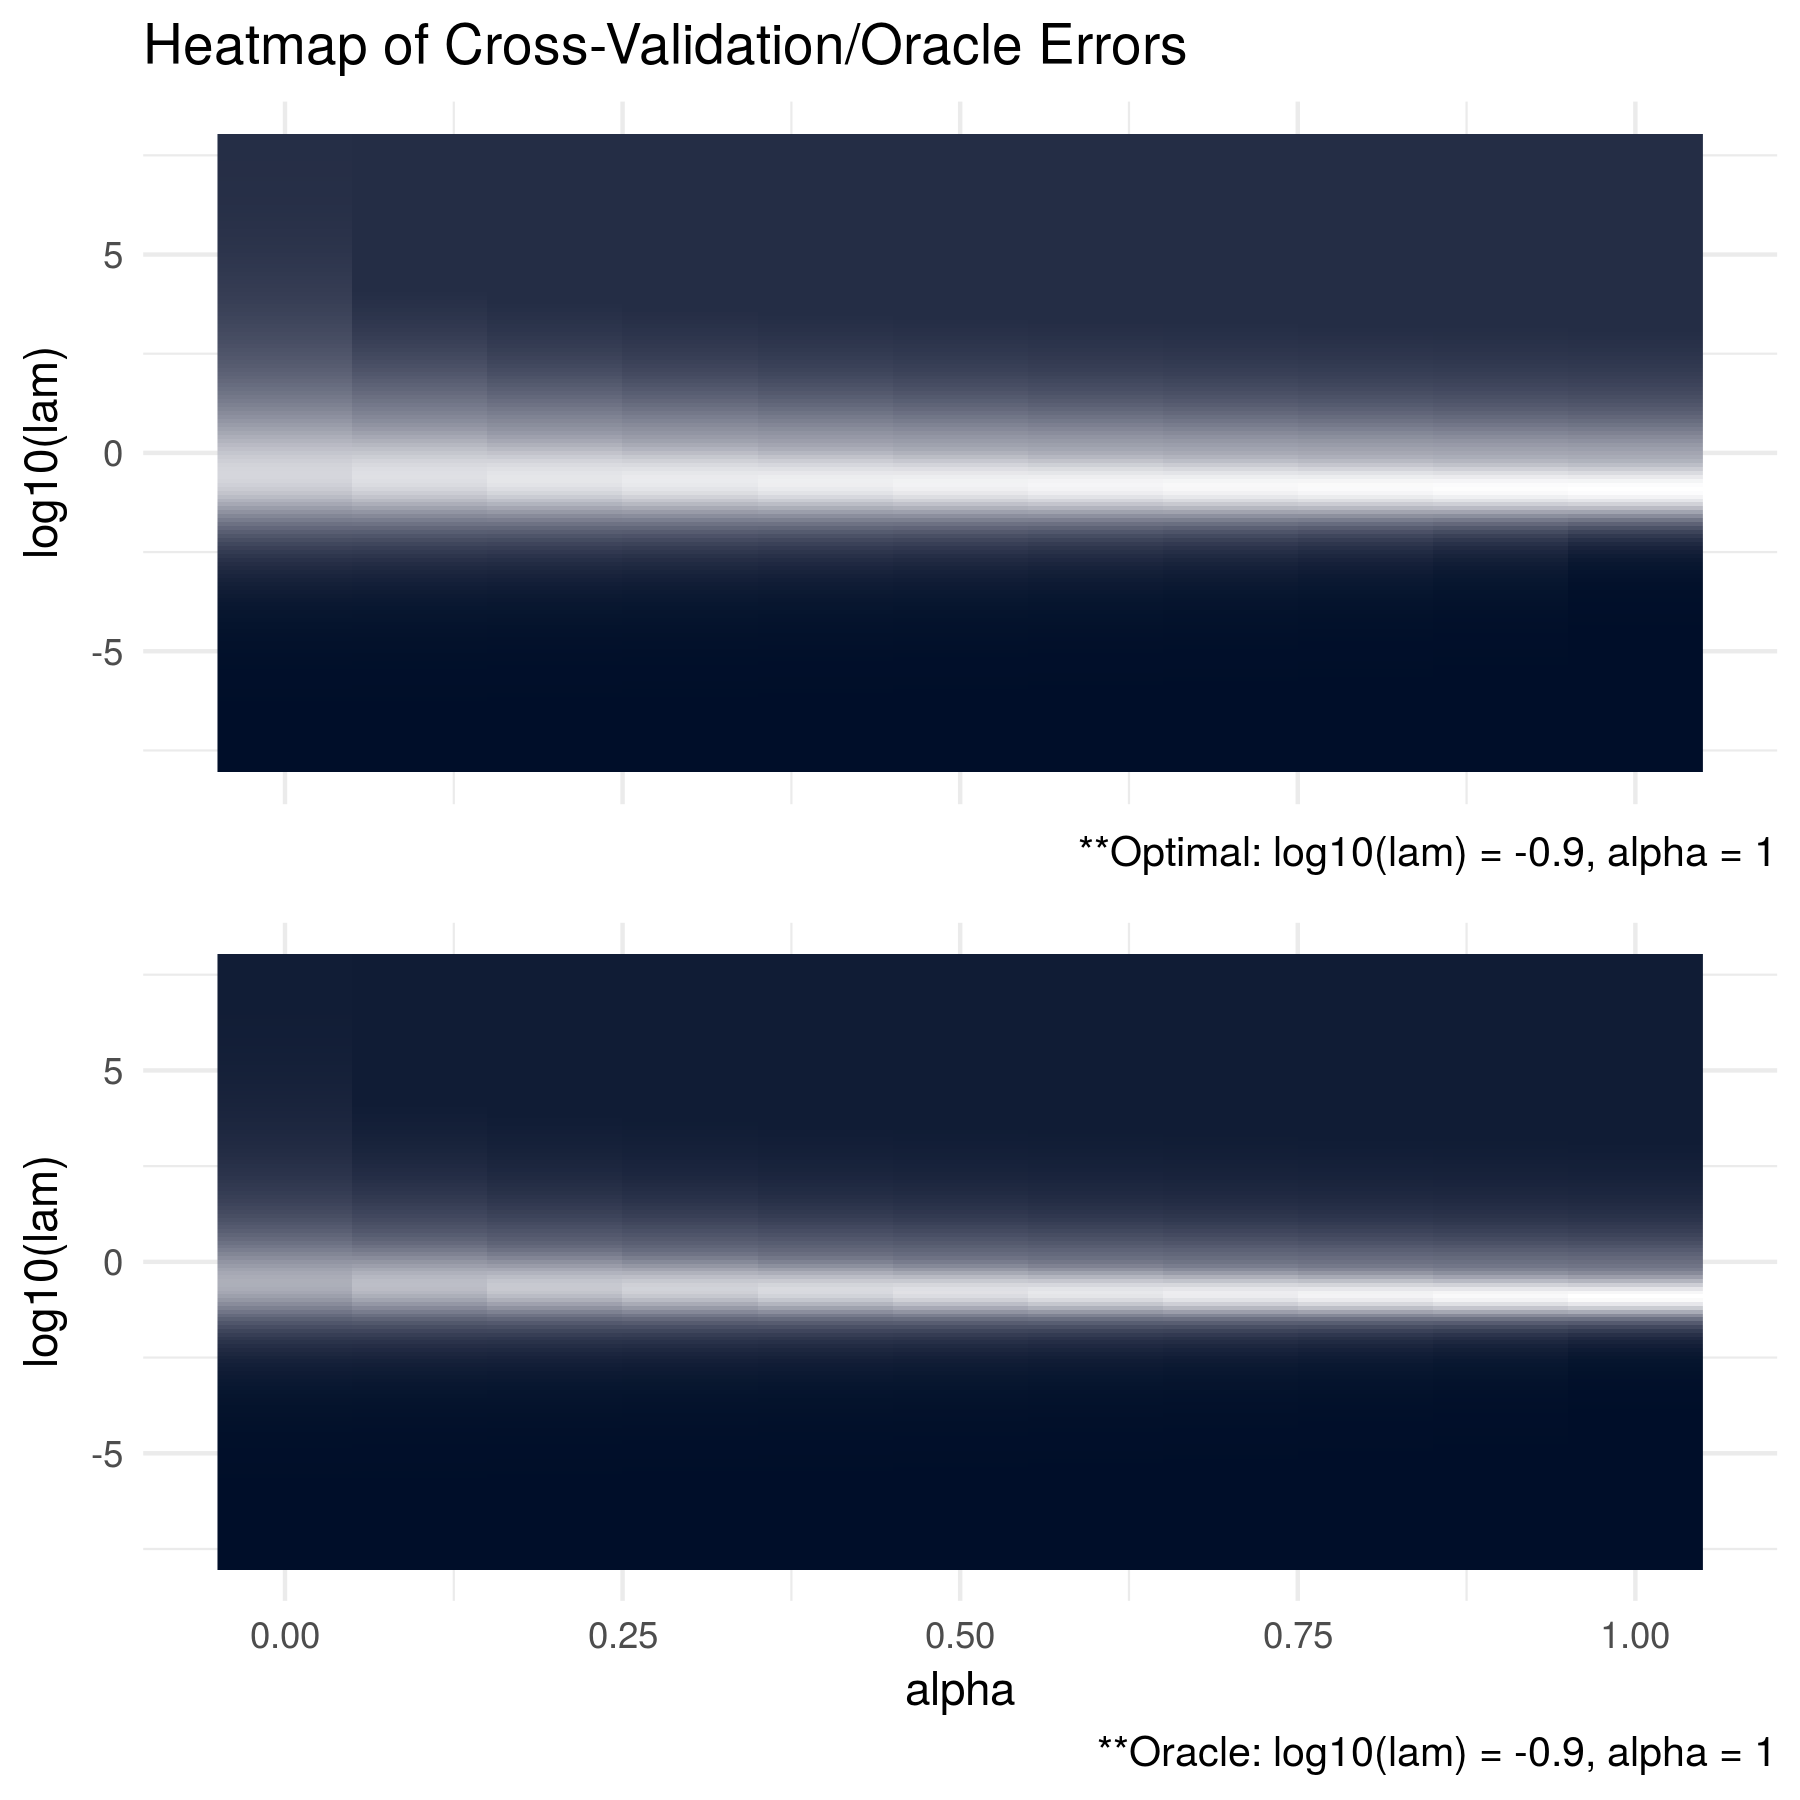
\includegraphics{images/repsKLtridiag_N50_P100.png}

\vspace{0.5cm}

\begin{Shaded}
\begin{Highlighting}[]
\CommentTok{# generate covariance matrix}
\CommentTok{# (can confirm inverse is tri-diagonal)}
\NormalTok{S =}\StringTok{ }\KeywordTok{matrix}\NormalTok{(}\DecValTok{0}\NormalTok{, }\DataTypeTok{nrow =} \DecValTok{100}\NormalTok{, }\DataTypeTok{ncol =} \DecValTok{100}\NormalTok{)}
\ControlFlowTok{for}\NormalTok{ (i }\ControlFlowTok{in} \DecValTok{1}\OperatorTok{:}\DecValTok{100}\NormalTok{)\{}
  \ControlFlowTok{for}\NormalTok{ (j }\ControlFlowTok{in} \DecValTok{1}\OperatorTok{:}\DecValTok{100}\NormalTok{)\{}
\NormalTok{    S[i, j] =}\StringTok{ }\FloatTok{0.7}\OperatorTok{^}\KeywordTok{abs}\NormalTok{(i }\OperatorTok{-}\StringTok{ }\NormalTok{j)}
\NormalTok{  \}}
\NormalTok{\}}

\CommentTok{# generate data}
\NormalTok{Z =}\StringTok{ }\KeywordTok{matrix}\NormalTok{(}\KeywordTok{rnorm}\NormalTok{(}\DecValTok{10}\OperatorTok{*}\DecValTok{50}\NormalTok{), }\DataTypeTok{nrow =} \DecValTok{50}\NormalTok{, }\DataTypeTok{ncol =} \DecValTok{10}\NormalTok{)}
\NormalTok{out =}\StringTok{ }\KeywordTok{eigen}\NormalTok{(S, }\DataTypeTok{symmetric =} \OtherTok{TRUE}\NormalTok{)}
\NormalTok{S.sqrt =}\StringTok{ }\NormalTok{out}\OperatorTok{$}\NormalTok{vectors }\OperatorTok\StringTok{ }\KeywordTok{diag}\NormalTok{(out}\OperatorTok{$}\NormalTok{values}\OperatorTok{^}\FloatTok{0.5}\NormalTok{) }\OperatorTok\StringTok{ }\KeywordTok{t}\NormalTok{(out}\OperatorTok{$}\NormalTok{vectors)}
\NormalTok{X =}\StringTok{ }\NormalTok{Z }\OperatorTok\StringTok{ }\NormalTok{S.sqrt}
\end{Highlighting}
\end{Shaded}

\hypertarget{benchmark}{%
\chapter{Benchmark}\label{benchmark}}

Below we benchmark the various functions contained in
\texttt{ADMMsigma}. We can see that \texttt{ADMMsigma} (at the default
tolerance) offers comparable computation time to the popular
\texttt{glasso} R package.

\hypertarget{computer-specs}{%
\subsection{Computer Specs:}\label{computer-specs}}

\begin{itemize}
\tightlist
\item
  MacBook Pro (Late 2016)
\item
  Processor: 2.9 GHz Intel Core i5
\item
  Memory: 8GB 2133 MHz
\item
  Graphics: Intel Iris Graphics 550
\end{itemize}

\vspace{0.5cm}

\begin{Shaded}
\begin{Highlighting}[]
\KeywordTok{library}\NormalTok{(ADMMsigma)}
\KeywordTok{library}\NormalTok{(microbenchmark)}

\CommentTok{# generate data from tri-diagonal (sparse) matrix compute covariance matrix}
\CommentTok{# (can confirm inverse is tri-diagonal)}
\NormalTok{S =}\StringTok{ }\KeywordTok{matrix}\NormalTok{(}\DecValTok{0}\NormalTok{, }\DataTypeTok{nrow =} \DecValTok{100}\NormalTok{, }\DataTypeTok{ncol =} \DecValTok{100}\NormalTok{)}

\ControlFlowTok{for}\NormalTok{ (i }\ControlFlowTok{in} \DecValTok{1}\OperatorTok{:}\DecValTok{100}\NormalTok{) \{}
    \ControlFlowTok{for}\NormalTok{ (j }\ControlFlowTok{in} \DecValTok{1}\OperatorTok{:}\DecValTok{100}\NormalTok{) \{}
\NormalTok{        S[i, j] =}\StringTok{ }\FloatTok{0.7}\OperatorTok{^}\NormalTok{(}\KeywordTok{abs}\NormalTok{(i }\OperatorTok{-}\StringTok{ }\NormalTok{j))}
\NormalTok{    \}}
\NormalTok{\}}

\CommentTok{# generate 1000 x 100 matrix with rows drawn from iid N_p(0, S)}
\KeywordTok{set.seed}\NormalTok{(}\DecValTok{123}\NormalTok{)}
\NormalTok{Z =}\StringTok{ }\KeywordTok{matrix}\NormalTok{(}\KeywordTok{rnorm}\NormalTok{(}\DecValTok{1000} \OperatorTok{*}\StringTok{ }\DecValTok{100}\NormalTok{), }\DataTypeTok{nrow =} \DecValTok{1000}\NormalTok{, }\DataTypeTok{ncol =} \DecValTok{100}\NormalTok{)}
\NormalTok{out =}\StringTok{ }\KeywordTok{eigen}\NormalTok{(S, }\DataTypeTok{symmetric =} \OtherTok{TRUE}\NormalTok{)}
\NormalTok{S.sqrt =}\StringTok{ }\NormalTok{out}\OperatorTok{$}\NormalTok{vectors }\OperatorTok\StringTok{ }\KeywordTok{diag}\NormalTok{(out}\OperatorTok{$}\NormalTok{values}\OperatorTok{^}\FloatTok{0.5}\NormalTok{) }\OperatorTok\StringTok{ }\KeywordTok{t}\NormalTok{(out}\OperatorTok{$}\NormalTok{vectors)}
\NormalTok{X =}\StringTok{ }\NormalTok{Z }\OperatorTok\StringTok{ }\NormalTok{S.sqrt}


\CommentTok{# glasso (for comparison)}
\KeywordTok{microbenchmark}\NormalTok{(glasso}\OperatorTok{::}\KeywordTok{glasso}\NormalTok{(}\DataTypeTok{s =}\NormalTok{ S, }\DataTypeTok{rho =} \FloatTok{0.1}\NormalTok{))}
\end{Highlighting}
\end{Shaded}

\begin{verbatim}
## Unit: milliseconds
##                              expr      min       lq     mean   median
##  glasso::glasso(s = S, rho = 0.1) 49.46673 53.37757 58.35196 55.90935
##        uq      max neval
##  60.77517 92.68082   100
\end{verbatim}

\begin{Shaded}
\begin{Highlighting}[]
\CommentTok{# benchmark ADMMsigma - default tolerance}
\KeywordTok{microbenchmark}\NormalTok{(}\KeywordTok{ADMMsigma}\NormalTok{(}\DataTypeTok{S =}\NormalTok{ S, }\DataTypeTok{lam =} \FloatTok{0.1}\NormalTok{, }\DataTypeTok{alpha =} \DecValTok{1}\NormalTok{, }\DataTypeTok{tol.abs =} \FloatTok{1e-04}\NormalTok{, }\DataTypeTok{tol.rel =} \FloatTok{1e-04}\NormalTok{, }
    \DataTypeTok{trace =} \StringTok{"none"}\NormalTok{))}
\end{Highlighting}
\end{Shaded}

\begin{verbatim}
## Unit: milliseconds
##                                                                                           expr
##  ADMMsigma(S = S, lam = 0.1, alpha = 1, tol.abs = 1e-04, tol.rel = 1e-04,      trace = "none")
##      min       lq     mean   median       uq      max neval
##  77.2134 83.51351 89.71565 85.37738 94.37814 126.0049   100
\end{verbatim}

\begin{Shaded}
\begin{Highlighting}[]
\CommentTok{# benchmark ADMMsigma - tolerance 1e-8}
\KeywordTok{microbenchmark}\NormalTok{(}\KeywordTok{ADMMsigma}\NormalTok{(}\DataTypeTok{S =}\NormalTok{ S, }\DataTypeTok{lam =} \FloatTok{0.1}\NormalTok{, }\DataTypeTok{alpha =} \DecValTok{1}\NormalTok{, }\DataTypeTok{tol.abs =} \FloatTok{1e-08}\NormalTok{, }\DataTypeTok{tol.rel =} \FloatTok{1e-08}\NormalTok{, }
    \DataTypeTok{trace =} \StringTok{"none"}\NormalTok{))}
\end{Highlighting}
\end{Shaded}

\begin{verbatim}
## Unit: milliseconds
##                                                                                           expr
##  ADMMsigma(S = S, lam = 0.1, alpha = 1, tol.abs = 1e-08, tol.rel = 1e-08,      trace = "none")
##       min       lq     mean   median       uq      max neval
##  258.5389 261.5402 272.3741 267.8829 274.7276 353.4726   100
\end{verbatim}

\begin{Shaded}
\begin{Highlighting}[]
\CommentTok{# benchmark ADMMsigma CV - default parameter grid}
\KeywordTok{microbenchmark}\NormalTok{(}\KeywordTok{ADMMsigma}\NormalTok{(X, }\DataTypeTok{trace =} \StringTok{"none"}\NormalTok{), }\DataTypeTok{times =} \DecValTok{5}\NormalTok{)}
\end{Highlighting}
\end{Shaded}

\begin{verbatim}
## Unit: seconds
##                          expr      min       lq     mean   median       uq
##  ADMMsigma(X, trace = "none") 8.338241 8.341611 8.536446 8.472933 8.515822
##       max neval
##  9.013621     5
\end{verbatim}

\begin{Shaded}
\begin{Highlighting}[]
\CommentTok{# benchmark ADMMsigma parallel CV}
\KeywordTok{microbenchmark}\NormalTok{(}\KeywordTok{ADMMsigma}\NormalTok{(X, }\DataTypeTok{cores =} \DecValTok{3}\NormalTok{, }\DataTypeTok{trace =} \StringTok{"none"}\NormalTok{), }\DataTypeTok{times =} \DecValTok{5}\NormalTok{)}
\end{Highlighting}
\end{Shaded}

\begin{verbatim}
## Unit: seconds
##                                     expr      min       lq     mean
##  ADMMsigma(X, cores = 3, trace = "none") 9.285137 9.315978 9.470666
##   median       uq      max neval
##  9.40943 9.426579 9.916207     5
\end{verbatim}

\begin{Shaded}
\begin{Highlighting}[]
\CommentTok{# benchmark ADMMsigma CV - likelihood convergence criteria}
\KeywordTok{microbenchmark}\NormalTok{(}\KeywordTok{ADMMsigma}\NormalTok{(X, }\DataTypeTok{crit =} \StringTok{"loglik"}\NormalTok{, }\DataTypeTok{trace =} \StringTok{"none"}\NormalTok{), }\DataTypeTok{times =} \DecValTok{5}\NormalTok{)}
\end{Highlighting}
\end{Shaded}

\begin{verbatim}
## Unit: seconds
##                                           expr      min       lq     mean
##  ADMMsigma(X, crit = "loglik", trace = "none") 7.028816 7.121599 7.185927
##    median       uq      max neval
##  7.181803 7.277249 7.320166     5
\end{verbatim}

\begin{Shaded}
\begin{Highlighting}[]
\CommentTok{# benchmark RIDGEsigma CV}
\KeywordTok{microbenchmark}\NormalTok{(}\KeywordTok{RIDGEsigma}\NormalTok{(X, }\DataTypeTok{lam =} \DecValTok{10}\OperatorTok{^}\KeywordTok{seq}\NormalTok{(}\OperatorTok{-}\DecValTok{8}\NormalTok{, }\DecValTok{8}\NormalTok{, }\FloatTok{0.01}\NormalTok{), }\DataTypeTok{trace =} \StringTok{"none"}\NormalTok{), }\DataTypeTok{times =} \DecValTok{5}\NormalTok{)}
\end{Highlighting}
\end{Shaded}

\begin{verbatim}
## Unit: seconds
##                                                      expr      min
##  RIDGEsigma(X, lam = 10^seq(-8, 8, 0.01), trace = "none") 12.22374
##        lq     mean   median       uq      max neval
##  12.37326 12.93705 13.01892 13.04356 14.02577     5
\end{verbatim}

\bibliography{lib.bib}

\end{document}
